\documentclass[preprint,aps,pra,onecolumn]{revtex4-1} %reprint
%\tightenlines

%\draft
\usepackage{etex}
\usepackage{amsmath}
\usepackage{bm}
\usepackage{bbm}
\usepackage{listings}
% % \textwidth 16cm \textheight 23.5cm
% \renewcommand{\baselinestretch}{1.2}
\usepackage{graphicx}
\usepackage{graphics}
\usepackage{epsfig}
\usepackage{color}
\usepackage{multirow}
\usepackage[colorlinks]{hyperref}
\usepackage{fancyhdr}
\usepackage{calc}
\usepackage{natbib} %[numbers]
\usepackage{bibentry}
% underline tool
\usepackage[normalem]{ulem}
\usepackage[usenames,dvipsnames]{xcolor}
%\uline{foo}	Underlines foo
%\uuline{foo}	Double underlines foo
%\uwave{foo}	Underlines foo with a wavy line
%\sout{foo}	Strikesout foo
%\xout{foo}	Crosses out foo with ¡®/6¤7¡¯
% triple lines in colors
\makeatletter
\newcommand\uuuline{\bgroup\markoverwith%
   {%
     \textcolor{red}{\rule[-0.5ex]{2pt}{0.4pt}}%
     \llap{\textcolor{blue}{\rule[-0.7ex]{2pt}{0.4pt}}}%
     \llap{\textcolor{green}{\rule[-0.9ex]{2pt}{0.4pt}}}%
   }%
   \ULon}
\makeatother


\usepackage{amsmath,soul} % underline with a number
% usage example: $\underset{4}{\text{\ul{This is short text}}}$
% another package to use, but did not work for me.
% From: http://tex.stackexchange.com/questions/45341/labeling-underlined-text-over-multiple-lines
%\usepackage{soulpos}
%\ulposdef{\ulnumaux}{%
%   $\underset{\saveulnum}{\rule[-.7ex]{\ulwidth}{.4pt}}$}
%
%\newcommand{\ulnum}[2]{%
%  \def\saveulnum{#1}%
%  \ulnumaux{#2}}

% todo list and commands
\usepackage{todonotes}
%% to avoid the conflict with amths package % not working
%\makeatletter
%\providecommand\@dotsep{5}
%\makeatother
%\listoftodos\relax
\usepackage{makeidx}
\allowdisplaybreaks
% for eps transfering to pdf.
\usepackage[update,prepend]{epstopdf}
\usepackage{ifpdf}

\ifpdf
   \usepackage{graphicx}
   \usepackage{epstopdf}
   \epstopdfsetup{suffix=}
   \DeclareGraphicsRule{.eps}{pdf}{.pdf}{`epstopdf #1}
   \pdfcompresslevel=9
\else
   \usepackage{graphicx}
\fi
% subfig
%\usepackage{mwe}
\usepackage{subfig}
% to fix a figure's position using [H] option of thec figure.
\usepackage{float}
% to use \lesssim and other math symbols
\usepackage{amssymb}


% self-defined short-cuts and commands

% packages we need for judging the operating system
% compile your tex file with option -shell-escape is required: 
% e.g. xelatex -shell-escape file.tex
\usepackage{pdftexcmds}
\usepackage{catchfile}
\usepackage{ifluatex}
\usepackage{ifplatform}

% self-definition for short hand

% symbols and math operators
\DeclareMathOperator{\spn}{span}
\DeclareMathOperator{\tr}{tr}
% definition of grammars % formats related
\definecolor{MyDarkGreen}{rgb}{0.0,0.4,0.0}
\newcommand{\greek}[1]{{\selectlanguage{greek}#1}} % will look for grmn font: tlmgr install cbfonts (65 MB)

% functions
\newcommand{\sn}{\mathrm{sn}}
\newcommand{\cn}{\mathrm{cn}}
\newcommand{\dn}{\mathrm{dn}}

% constants
\newcommand{\invtpi}{\frac{1}{2\pi}}

% vectors and tensors
\def\en{\mathbf{e}_n}
\def\eye{\mathbf{I}}
\newcommand\lvec[1]{\accentset{\leftarrow}{#1}}
% math font
\newcommand{\bmc}[1]{\boldsymbol{\mathcal{#1}}}

% derivatives and integrals
% ordinary derivatives
\newcommand{\drv}{\mathrm{d}}
\newcommand{\dt}[1]{\frac{{\mathrm d} {#1}}{{\mathrm d}t}}
\newcommand{\dx}[1]{\frac{{\mathrm d} {#1}}{{\mathrm d}x}}
\newcommand{\dtau}{\frac{{\mathrm d} }{{\mathrm d}\tau}}
\newcommand{\dd}[2]{\frac{{\mathrm d} {#1}}{{\mathrm d} {#2}}}
\newcommand{\sdt}[1]{\frac{{\mathrm d}^2 {#1}}{{\mathrm d}t^2}}
\newcommand{\sdx}[1]{\frac{{\mathrm d}^2 {#1}}{{\mathrm d}x^2}}
\newcommand{\sdd}[2]{\frac{{\mathrm d}^2 {#1}}{{\mathrm d}{#2}^2}}
\newcommand{\ddn}[3]{\frac{{\mathrm d}^{#1} #2}{{\mathrm d} #3 ^{#1}}}

% partial derivatives
\newcommand{\pt}[1]{\frac{\partial {#1}}{\partial t}}
\newcommand{\px}[1]{\frac{\partial {#1}}{\partial x}}
\newcommand{\pp}[2]{\frac{\partial {#1}}{\partial {#2}}}
\newcommand{\spt}[1]{\frac{\partial^2 {#1}}{\partial t^2}}
\newcommand{\spx}[1]{\frac{\partial^2 {#1}}{\partial x^2}}
\newcommand{\spp}[2]{\frac{\partial^2 {#1}}{\partial {#2}^2}}
\newcommand{\ppn}[3]{\frac{\partial^{#1} #2}{\partial #3 ^{#1}}}
% integrals
\newcommand{\intl}[2]{\int_0^\infty\! #1 \mathrm{d}#2}
\newcommand{\intf}[2]{\int_{-\infty}^\infty\! #1 \mathrm{d}#2}


% quantum operators
\newcommand{\ssp}{\braket{\sigma^{+}(t)\sigma^{-}(t)}}
\newcommand{\aap}{\braket{a^{\dagger}(t)a(t)}}
\newcommand{\as}{\braket{a^{\dagger}(t)\sigma^{-}(t)}}
\newcommand{\sa}{\braket{a(t)\sigma^{+}(t)}}
\newcommand{\Hssp}{\braket{\sigma^{+}\sigma^{-}}}
\newcommand{\Haap}{\braket{a^{\dagger}a}}
\newcommand{\Has}{\braket{a^{\dagger}\sigma^{-}}}
\newcommand{\Hsa}{\braket{a\sigma^{+}}}
\newcommand{\adag}{a^{\dagger}}
\newcommand{\sigm}{\sigma^{-}}
\newcommand{\sigp}{\sigma^{+}}
\newcommand{\sigz}{\sigma^{z}}
\newcommand{\gp}{\gamma^{\prime}}
\newcommand{\oal}{\omega_a-\omega_0}
\newcommand{\ocl}{\omega_c-\omega_0}


% Green function related
\def\GFT{\overline{\bf G}}
\def\IT{\overline{\bf I}}
\def\TT{\overline{\bf T}}
\def\MT{\overline{\bf M}}
\def\AT{\overline{\bf A}}
\def\BT{\overline{\bf B}}
\def\fT{\overline{\bf f}}
\def\LT{\overline{\bf L}}
\def\alphaT{\overline{\bf \alpha}}
\def\GFTr{\overline{\bf G}\left(\mathbf{r},\mathbf{r}'\right)}
\def\GFTrw{\overline{\bf G}\left(\mathbf{r},\mathbf{r}';\omega\right)}
\def\rarg{\left(\mathbf{r}\right)}
\def\rargw{\left(\mathbf{r};\omega\right)}
\def\rrarg{\left(\mathbf{r},\mathbf{r}'\right)}
\def\rrargw{\left(\mathbf{r},\mathbf{r}';\omega\right)}
\def\rk{\left(\mathbf{r}_k\right)}
\def\rn{\left(\mathbf{r}_n\right)}
\def\rnrn{\left(\mathbf{r}_n,\mathbf{r}_n\right)}
\def\rnrk{\left(\mathbf{r}_n,\mathbf{r}_k\right)}
\def\rkrk{\left(\mathbf{r}_k,\mathbf{r}_k\right)}
\def\rkrn{\left(\mathbf{r}_k,\mathbf{r}_n\right)}
\def\br{\mathbf{r}}
\def\Erw{\hat{\mathbf{E}}(\mathbf{r},\omega)}
\def\E0{\hat{\mathbf{E}}^{(0)}(\mathbf{r},\omega)}
\def\Arw{\hat{\mathbf{A}}(\mathbf{r},\omega)}
\def\Snw{\hat{\mathbf{S}}_n(\omega)}
\def\Unw{\mathbf{U}_n(\omega)}
\def\unw{U_n(\omega)}
\def\Alphanw{{\bm \alpha}_n(\omega)}
\def\Krrw{\mathbf{K}(\mathbf{r},\mathbf{r}',\omega)}
\def\Krrnw{\mathbf{K}(\mathbf{r},\mathbf{r}_n,\omega)}
\def\GTrrw{\mathbf{G}^T(\mathbf{r},\mathbf{r}',\omega)}
\def\Grrw{\mathbf{G}(\mathbf{r},\mathbf{r}',\omega)}
\def\Gn{\mathbf{G}^n}
\def\Gm1{\mathbf{G}^{n-1}}
\def\GN{\mathbf{G}^N}
\def\G0{\mathbf{G}^0}
\def\G1{\mathbf{G}^1}
\def\Gi{\mathbf{G}^i}
\def\flamr{\mathbf{f}_\lambda(\mathbf{r})}
\def\rrn{\mathbf{r},\mathbf{r}_n}
\def\rnrn{\mathbf{r}_n,\mathbf{r}_n}
\def\rr{\mathbf{r},\mathbf{r}'}


% braket.sty          Macros for Dirac bra-ket <|> notation and sets {|}
%
\def\bra#1{\langle{#1}\rvert}%{\mathinner{\langle{#1}\rvert}}
\def\ket#1{\lvert{#1}\rangle}%{\mathinner{\lvert{#1}\rangle}}
\def\braket#1{\mathinner{\langle{#1}\rangle}}
\def\Bra#1{\left<#1\right|}
\def\Ket#1{\left|#1\right>}
{\catcode`\|=\active
  \gdef\Braket#1{\left<\mathcode`\|"8000\let|\BraVert {#1}\right>}}
\def\BraVert{\egroup\,\mid@vertical\,\bgroup}
{\catcode`\|=\active
  \gdef\set#1{\mathinner{\lbrace\,{\mathcode`\|"8000\let|\midvert #1}\,\rbrace}}
  \gdef\Set#1{\left\{\:{\mathcode`\|"8000\let|\SetVert #1}\:\right\}}}
\def\midvert{\egroup\mid\bgroup}
\def\SetVert{\egroup\;\mid@vertical\;\bgroup}
% Some stuff deleted
% Macros for Dirac bra-ket <|> notation
%\def\bra#1{\mathinner{\langle{#1}|}}
%\def\ket#1{\mathinner{|{#1}\rangle}}
\def\Braket#1#2{\mathinner{\langle{#1}\! \mid\! {#2} \rangle}}
\def\ketbra#1{\ket{#1}\!\!\bra{#1}}
\newcommand{\Ketbra}[2]{\ket{#1}\!\!\bra{#2}}
\def\sandwich#1#2{\bra{#1}\! #2 \! \ket{#1}}
\def\Sandwich#1#2#3{\bra{#1}\! #2\! \ket{#3}}
%
% END  braket.sty     Macros for Dirac bra-ket <|> notation and sets {|}


%% Ben's shortcuts.
% Equation, citation, and labeling macros
%========================================================================================
\newcommand{\erf}[1]{Eq.~(\ref{#1})}
\newcommand{\frf}[1]{Fig.~\ref{#1}}
\newcommand{\srf}[1]{Sec.~\ref{#1}}
\newcommand{\nn}{\nonumber}
\newcommand{\mbf}[1]{\mathbf{#1}}
%========================================================================================
% General quantum mechanics macros
%========================================================================================
\newcommand{\ip}[2]{\langle{#1}|{#2}\rangle}
\newcommand{\op}[2]{\ket{#1}\bra{#2}}
\newcommand{\enavg}[1]{\mathrm{E}\sq{#1}}
\newcommand{\gravg}[1]{\mathbb{E}\sq{#1}}
\newcommand{\expt}[1]{\langle{#1}\rangle}
\newcommand{\dg}{^\dagger}
\newcommand{\smallfrac}[2]{\mbox{$\frac{#1}{#2}$}}
\newcommand{\emn}[1]{ \mathbbm{E}_{#1} }
\newcommand{\Tr}{\mbox{Tr}}
%\newcommand{\tensor}[1]{\boldsymbol{#1}}%{\overset{\leftrightarrow}{#1}}
%========================================================================================
% Famous physicists
%========================================================================================
\newcommand{\sch}{Schr\"odinger}
\newcommand{\hei}{Heisenberg }
\newcommand{\ein}{Einstein }
\newcommand{\str}{Stratonovich }
%========================================================================================
% Dirac notation and commutators
%========================================================================================
\newcommand{\norm}[1]{\lvert #1 \rvert}
\newcommand{\opnorm}[1]{\lVert #1 \rVert}
%\newcommand{\ket}[1]{\lvert #1 \rangle}
%\newcommand{\bra}[1]{\langle #1 \rvert}
\newcommand{\bravket}[2]{\langle\, #1\,\vert\, #2 \,\rangle}
\newcommand{\av}[1]{\left\langle #1 \right\rangle}
\newcommand{\proj}[1]{\ket{#1}\!\bra{#1}}
\newcommand{\commut}[2]{[\ssp #1,\,#2\ssp]}
\newcommand{\anticommut}[2]{\{\ssp #1,\,#2\ssp\}}
% big Dirac notation and commutators
\newcommand{\bnorm}[1]{\big\lvert #1 \big\rvert}
\newcommand{\bopnorm}[1]{\big\lVert #1 \big\rVert}
\newcommand{\bket}[1]{\big\lvert\, #1\, \big\rangle}
\newcommand{\bbra}[1]{\big\langle\, #1\, \big\rvert}
\newcommand{\bbraket}[2]{\big\langle\, #1\,\big\vert\, #2 \,\big\rangle}
\newcommand{\bav}[1]{\bigl\langle #1 \bigr\rangle}
\newcommand{\bproj}[1]{\bket{#1}\!\bbra{#1}}
\newcommand{\bcommut}[2]{\big[\ssp #1,\,#2\ssp\big]}
\newcommand{\banticommut}[2]{\big\{\ssp #1,\,#2\ssp\big\}}
% Big Dirac notation and commutators
\newcommand{\Bnorm}[1]{\Big\lvert #1 \Big\rvert}
\newcommand{\Bopnorm}[1]{\Big\lVert #1 \Big\rVert}
\newcommand{\Bket}[1]{\Big\lvert\, #1\, \Big\rangle}
\newcommand{\Bbra}[1]{\Big\langle\, #1\, \Big\rvert}
\newcommand{\Bbraket}[2]{\Big\langle\, #1\,\Big\vert\, #2 \,\Big\rangle}
\newcommand{\Bav}[1]{\Bigl\langle #1 \Bigr\rangle}
\newcommand{\Bproj}[1]{\Bket{#1}\!\Bbra{#1}}
\newcommand{\Bcommut}[2]{\Big[\ssp #1,\,#2\ssp\Big]}
\newcommand{\Banticommut}[2]{\Big\{\ssp #1,\,#2\ssp\Big\}}
%========================================================================================
% Nanofiber interface macros
%========================================================================================
\newcommand{\expect}[1]{\big\langle #1 \big\rangle}
\newcommand{\expects}[1]{\langle #1 \rangle}
\newcommand{\melement}[3]{\langle #1 \lvert #2 \rvert #3 \rangle}
\newcommand{\Ip}[2]{\left\langle {#1},{#2} \right\rangle}
\newcommand{\modsq}[1]{\lvert #1 \rvert^2}
\newcommand{\normsq}[1]{\lVert #1 \rVert^2}
\newcommand{\grad}{\nabla}
\newcommand{\partialD}[2]{\frac{\partial #1}{\partial #2}}

\newcommand{\peakprobe}{\mathcal{E}_0}
\newcommand{\eff}{\text{eff}}
\newcommand{\varFz}{\big( \Delta F_z^{0} \big)^2}
\newcommand{\varFzText}{( \Delta F_z^{0} )^2}
\newcommand{\varFzLG}{( \Delta F_z^{00} )^2}

\newcommand{\rperp}{\mathbf{r}_\perp}
\newcommand{\talphan}{\overset{\leftrightarrow}{\alpha}{}^{(n)}}
\newcommand{\talphanOp}{\hat{\overset{\leftrightarrow}{\alpha}}{}^{(n)}}

%\newcommand{\Cstrength}{ \chi^{(1)}\sqrt{ \dot{N}_L } }
%\newcommand{\CstrengthSq}{ \big(\chi^{(1)} \big)^2 \dot{N}_L }
\newcommand{\Cstrength}{ \sqrt{\kappa} }
\newcommand{\CstrengthSq}{ \kappa }
%========================================================================================
%  Spacing macros
%========================================================================================
%\newcommand{\ssp}{\hspace{0.4pt}}%small horizontal space
\newcommand{\nsp}{\hspace{-0.7pt}}%negative horizontal space
%========================================================================================




% For faster processing, load Matlab syntax for listings
\lstloadlanguages{Matlab}% use listings package
\lstset{language=Matlab,
        frame=single,
        basicstyle=\small\ttfamily,
        keywordstyle=[1]\color{Blue}\bf,
        keywordstyle=[2]\color{Purple},
        keywordstyle=[3]\color{Blue}\underbar,
        identifierstyle=,
        commentstyle=\usefont{T1}{pcr}{m}{sl}\color{MyDarkGreen}\small,
        stringstyle=\color{Purple},
        showstringspaces=false,
        tabsize=5,
        % Put standard MATLAB functions not included in the default
        % language here
        morekeywords={xlim,ylim,var,alpha,factorial,poissrnd,normpdf,normcdf},
        % Put MATLAB function parameters here
        morekeywords=[2]{on, off, interp},
        % Put user defined functions here
        morekeywords=[3]{FindESS},
        morecomment=[l][\color{Blue}]{...},
        numbers=left,
        firstnumber=1,
        numberstyle=\tiny\color{Blue},
        stepnumber=5
        }
        
        
        
% Includes a figure
% The first parameter is the label, which is also the name of the figure
%   with or without the extension (e.g., .eps, .fig, .png, .gif, etc.)
%   IF NO EXTENSION IS GIVEN, LaTeX will look for the most appropriate one.
%   This means that if a DVI (or PS) is being produced, it will look for
%   an eps. If a PDF is being produced, it will look for nearly anything
%   else (gif, jpg, png, et cetera). Because of this, when I generate figures
%   I typically generate an eps and a png to allow me the most flexibility
%   when rendering my document.
% The second parameter is the width of the figure normalized to column width
%   (e.g. 0.5 for half a column, 0.75 for 75% of the column)
% The third parameter is the caption.
\newcommand{\scalefig}[3]{
  \begin{figure}[ht!]
    % Requires \usepackage{graphicx}
    \centering
    \includegraphics[width=#2\columnwidth]{#1}
    %%% I think \captionwidth (see above) can go away as long as
    %%% \centering is above
    %\captionwidth{#2\columnwidth}%
    \caption{#3}
    \label{#1}
  \end{figure}}
% judge platform and include correct definiation package
%\ifwindows
%	%% self-definition for short hand

% symbols and math operators
\DeclareMathOperator{\spn}{span}
\DeclareMathOperator{\tr}{tr}
% definition of grammars % formats related
\definecolor{MyDarkGreen}{rgb}{0.0,0.4,0.0}
\newcommand{\greek}[1]{{\selectlanguage{greek}#1}} % will look for grmn font: tlmgr install cbfonts (65 MB)

% functions
\newcommand{\sn}{\mathrm{sn}}
\newcommand{\cn}{\mathrm{cn}}
\newcommand{\dn}{\mathrm{dn}}

% constants
\newcommand{\invtpi}{\frac{1}{2\pi}}

% vectors and tensors
\def\en{\mathbf{e}_n}
\def\eye{\mathbf{I}}
\newcommand\lvec[1]{\accentset{\leftarrow}{#1}}
% math font
\newcommand{\bmc}[1]{\boldsymbol{\mathcal{#1}}}

% derivatives and integrals
% ordinary derivatives
\newcommand{\drv}{\mathrm{d}}
\newcommand{\dt}[1]{\frac{{\mathrm d} {#1}}{{\mathrm d}t}}
\newcommand{\dx}[1]{\frac{{\mathrm d} {#1}}{{\mathrm d}x}}
\newcommand{\dtau}{\frac{{\mathrm d} }{{\mathrm d}\tau}}
\newcommand{\dd}[2]{\frac{{\mathrm d} {#1}}{{\mathrm d} {#2}}}
\newcommand{\sdt}[1]{\frac{{\mathrm d}^2 {#1}}{{\mathrm d}t^2}}
\newcommand{\sdx}[1]{\frac{{\mathrm d}^2 {#1}}{{\mathrm d}x^2}}
\newcommand{\sdd}[2]{\frac{{\mathrm d}^2 {#1}}{{\mathrm d}{#2}^2}}
\newcommand{\ddn}[3]{\frac{{\mathrm d}^{#1} #2}{{\mathrm d} #3 ^{#1}}}

% partial derivatives
\newcommand{\pt}[1]{\frac{\partial {#1}}{\partial t}}
\newcommand{\px}[1]{\frac{\partial {#1}}{\partial x}}
\newcommand{\pp}[2]{\frac{\partial {#1}}{\partial {#2}}}
\newcommand{\spt}[1]{\frac{\partial^2 {#1}}{\partial t^2}}
\newcommand{\spx}[1]{\frac{\partial^2 {#1}}{\partial x^2}}
\newcommand{\spp}[2]{\frac{\partial^2 {#1}}{\partial {#2}^2}}
\newcommand{\ppn}[3]{\frac{\partial^{#1} #2}{\partial #3 ^{#1}}}
% integrals
\newcommand{\intl}[2]{\int_0^\infty\! #1 \mathrm{d}#2}
\newcommand{\intf}[2]{\int_{-\infty}^\infty\! #1 \mathrm{d}#2}


% quantum operators
\newcommand{\ssp}{\braket{\sigma^{+}(t)\sigma^{-}(t)}}
\newcommand{\aap}{\braket{a^{\dagger}(t)a(t)}}
\newcommand{\as}{\braket{a^{\dagger}(t)\sigma^{-}(t)}}
\newcommand{\sa}{\braket{a(t)\sigma^{+}(t)}}
\newcommand{\Hssp}{\braket{\sigma^{+}\sigma^{-}}}
\newcommand{\Haap}{\braket{a^{\dagger}a}}
\newcommand{\Has}{\braket{a^{\dagger}\sigma^{-}}}
\newcommand{\Hsa}{\braket{a\sigma^{+}}}
\newcommand{\adag}{a^{\dagger}}
\newcommand{\sigm}{\sigma^{-}}
\newcommand{\sigp}{\sigma^{+}}
\newcommand{\sigz}{\sigma^{z}}
\newcommand{\gp}{\gamma^{\prime}}
\newcommand{\oal}{\omega_a-\omega_0}
\newcommand{\ocl}{\omega_c-\omega_0}


% Green function related
\def\GFT{\overline{\bf G}}
\def\IT{\overline{\bf I}}
\def\TT{\overline{\bf T}}
\def\MT{\overline{\bf M}}
\def\AT{\overline{\bf A}}
\def\BT{\overline{\bf B}}
\def\fT{\overline{\bf f}}
\def\LT{\overline{\bf L}}
\def\alphaT{\overline{\bf \alpha}}
\def\GFTr{\overline{\bf G}\left(\mathbf{r},\mathbf{r}'\right)}
\def\GFTrw{\overline{\bf G}\left(\mathbf{r},\mathbf{r}';\omega\right)}
\def\rarg{\left(\mathbf{r}\right)}
\def\rargw{\left(\mathbf{r};\omega\right)}
\def\rrarg{\left(\mathbf{r},\mathbf{r}'\right)}
\def\rrargw{\left(\mathbf{r},\mathbf{r}';\omega\right)}
\def\rk{\left(\mathbf{r}_k\right)}
\def\rn{\left(\mathbf{r}_n\right)}
\def\rnrn{\left(\mathbf{r}_n,\mathbf{r}_n\right)}
\def\rnrk{\left(\mathbf{r}_n,\mathbf{r}_k\right)}
\def\rkrk{\left(\mathbf{r}_k,\mathbf{r}_k\right)}
\def\rkrn{\left(\mathbf{r}_k,\mathbf{r}_n\right)}
\def\br{\mathbf{r}}
\def\Erw{\hat{\mathbf{E}}(\mathbf{r},\omega)}
\def\E0{\hat{\mathbf{E}}^{(0)}(\mathbf{r},\omega)}
\def\Arw{\hat{\mathbf{A}}(\mathbf{r},\omega)}
\def\Snw{\hat{\mathbf{S}}_n(\omega)}
\def\Unw{\mathbf{U}_n(\omega)}
\def\unw{U_n(\omega)}
\def\Alphanw{{\bm \alpha}_n(\omega)}
\def\Krrw{\mathbf{K}(\mathbf{r},\mathbf{r}',\omega)}
\def\Krrnw{\mathbf{K}(\mathbf{r},\mathbf{r}_n,\omega)}
\def\GTrrw{\mathbf{G}^T(\mathbf{r},\mathbf{r}',\omega)}
\def\Grrw{\mathbf{G}(\mathbf{r},\mathbf{r}',\omega)}
\def\Gn{\mathbf{G}^n}
\def\Gm1{\mathbf{G}^{n-1}}
\def\GN{\mathbf{G}^N}
\def\G0{\mathbf{G}^0}
\def\G1{\mathbf{G}^1}
\def\Gi{\mathbf{G}^i}
\def\flamr{\mathbf{f}_\lambda(\mathbf{r})}
\def\rrn{\mathbf{r},\mathbf{r}_n}
\def\rnrn{\mathbf{r}_n,\mathbf{r}_n}
\def\rr{\mathbf{r},\mathbf{r}'}


% braket.sty          Macros for Dirac bra-ket <|> notation and sets {|}
%
\def\bra#1{\langle{#1}\rvert}%{\mathinner{\langle{#1}\rvert}}
\def\ket#1{\lvert{#1}\rangle}%{\mathinner{\lvert{#1}\rangle}}
\def\braket#1{\mathinner{\langle{#1}\rangle}}
\def\Bra#1{\left<#1\right|}
\def\Ket#1{\left|#1\right>}
{\catcode`\|=\active
  \gdef\Braket#1{\left<\mathcode`\|"8000\let|\BraVert {#1}\right>}}
\def\BraVert{\egroup\,\mid@vertical\,\bgroup}
{\catcode`\|=\active
  \gdef\set#1{\mathinner{\lbrace\,{\mathcode`\|"8000\let|\midvert #1}\,\rbrace}}
  \gdef\Set#1{\left\{\:{\mathcode`\|"8000\let|\SetVert #1}\:\right\}}}
\def\midvert{\egroup\mid\bgroup}
\def\SetVert{\egroup\;\mid@vertical\;\bgroup}
% Some stuff deleted
% Macros for Dirac bra-ket <|> notation
%\def\bra#1{\mathinner{\langle{#1}|}}
%\def\ket#1{\mathinner{|{#1}\rangle}}
\def\Braket#1#2{\mathinner{\langle{#1}\! \mid\! {#2} \rangle}}
\def\ketbra#1{\ket{#1}\!\!\bra{#1}}
\newcommand{\Ketbra}[2]{\ket{#1}\!\!\bra{#2}}
\def\sandwich#1#2{\bra{#1}\! #2 \! \ket{#1}}
\def\Sandwich#1#2#3{\bra{#1}\! #2\! \ket{#3}}
%
% END  braket.sty     Macros for Dirac bra-ket <|> notation and sets {|}


%% Ben's shortcuts.
% Equation, citation, and labeling macros
%========================================================================================
\newcommand{\erf}[1]{Eq.~(\ref{#1})}
\newcommand{\frf}[1]{Fig.~\ref{#1}}
\newcommand{\srf}[1]{Sec.~\ref{#1}}
\newcommand{\nn}{\nonumber}
\newcommand{\mbf}[1]{\mathbf{#1}}
%========================================================================================
% General quantum mechanics macros
%========================================================================================
\newcommand{\ip}[2]{\langle{#1}|{#2}\rangle}
\newcommand{\op}[2]{\ket{#1}\bra{#2}}
\newcommand{\enavg}[1]{\mathrm{E}\sq{#1}}
\newcommand{\gravg}[1]{\mathbb{E}\sq{#1}}
\newcommand{\expt}[1]{\langle{#1}\rangle}
\newcommand{\dg}{^\dagger}
\newcommand{\smallfrac}[2]{\mbox{$\frac{#1}{#2}$}}
\newcommand{\emn}[1]{ \mathbbm{E}_{#1} }
\newcommand{\Tr}{\mbox{Tr}}
%\newcommand{\tensor}[1]{\boldsymbol{#1}}%{\overset{\leftrightarrow}{#1}}
%========================================================================================
% Famous physicists
%========================================================================================
\newcommand{\sch}{Schr\"odinger}
\newcommand{\hei}{Heisenberg }
\newcommand{\ein}{Einstein }
\newcommand{\str}{Stratonovich }
%========================================================================================
% Dirac notation and commutators
%========================================================================================
\newcommand{\norm}[1]{\lvert #1 \rvert}
\newcommand{\opnorm}[1]{\lVert #1 \rVert}
%\newcommand{\ket}[1]{\lvert #1 \rangle}
%\newcommand{\bra}[1]{\langle #1 \rvert}
\newcommand{\bravket}[2]{\langle\, #1\,\vert\, #2 \,\rangle}
\newcommand{\av}[1]{\left\langle #1 \right\rangle}
\newcommand{\proj}[1]{\ket{#1}\!\bra{#1}}
\newcommand{\commut}[2]{[\ssp #1,\,#2\ssp]}
\newcommand{\anticommut}[2]{\{\ssp #1,\,#2\ssp\}}
% big Dirac notation and commutators
\newcommand{\bnorm}[1]{\big\lvert #1 \big\rvert}
\newcommand{\bopnorm}[1]{\big\lVert #1 \big\rVert}
\newcommand{\bket}[1]{\big\lvert\, #1\, \big\rangle}
\newcommand{\bbra}[1]{\big\langle\, #1\, \big\rvert}
\newcommand{\bbraket}[2]{\big\langle\, #1\,\big\vert\, #2 \,\big\rangle}
\newcommand{\bav}[1]{\bigl\langle #1 \bigr\rangle}
\newcommand{\bproj}[1]{\bket{#1}\!\bbra{#1}}
\newcommand{\bcommut}[2]{\big[\ssp #1,\,#2\ssp\big]}
\newcommand{\banticommut}[2]{\big\{\ssp #1,\,#2\ssp\big\}}
% Big Dirac notation and commutators
\newcommand{\Bnorm}[1]{\Big\lvert #1 \Big\rvert}
\newcommand{\Bopnorm}[1]{\Big\lVert #1 \Big\rVert}
\newcommand{\Bket}[1]{\Big\lvert\, #1\, \Big\rangle}
\newcommand{\Bbra}[1]{\Big\langle\, #1\, \Big\rvert}
\newcommand{\Bbraket}[2]{\Big\langle\, #1\,\Big\vert\, #2 \,\Big\rangle}
\newcommand{\Bav}[1]{\Bigl\langle #1 \Bigr\rangle}
\newcommand{\Bproj}[1]{\Bket{#1}\!\Bbra{#1}}
\newcommand{\Bcommut}[2]{\Big[\ssp #1,\,#2\ssp\Big]}
\newcommand{\Banticommut}[2]{\Big\{\ssp #1,\,#2\ssp\Big\}}
%========================================================================================
% Nanofiber interface macros
%========================================================================================
\newcommand{\expect}[1]{\big\langle #1 \big\rangle}
\newcommand{\expects}[1]{\langle #1 \rangle}
\newcommand{\melement}[3]{\langle #1 \lvert #2 \rvert #3 \rangle}
\newcommand{\Ip}[2]{\left\langle {#1},{#2} \right\rangle}
\newcommand{\modsq}[1]{\lvert #1 \rvert^2}
\newcommand{\normsq}[1]{\lVert #1 \rVert^2}
\newcommand{\grad}{\nabla}
\newcommand{\partialD}[2]{\frac{\partial #1}{\partial #2}}

\newcommand{\peakprobe}{\mathcal{E}_0}
\newcommand{\eff}{\text{eff}}
\newcommand{\varFz}{\big( \Delta F_z^{0} \big)^2}
\newcommand{\varFzText}{( \Delta F_z^{0} )^2}
\newcommand{\varFzLG}{( \Delta F_z^{00} )^2}

\newcommand{\rperp}{\mathbf{r}_\perp}
\newcommand{\talphan}{\overset{\leftrightarrow}{\alpha}{}^{(n)}}
\newcommand{\talphanOp}{\hat{\overset{\leftrightarrow}{\alpha}}{}^{(n)}}

%\newcommand{\Cstrength}{ \chi^{(1)}\sqrt{ \dot{N}_L } }
%\newcommand{\CstrengthSq}{ \big(\chi^{(1)} \big)^2 \dot{N}_L }
\newcommand{\Cstrength}{ \sqrt{\kappa} }
\newcommand{\CstrengthSq}{ \kappa }
%========================================================================================
%  Spacing macros
%========================================================================================
%\newcommand{\ssp}{\hspace{0.4pt}}%small horizontal space
\newcommand{\nsp}{\hspace{-0.7pt}}%negative horizontal space
%========================================================================================




% For faster processing, load Matlab syntax for listings
\lstloadlanguages{Matlab}% use listings package
\lstset{language=Matlab,
        frame=single,
        basicstyle=\small\ttfamily,
        keywordstyle=[1]\color{Blue}\bf,
        keywordstyle=[2]\color{Purple},
        keywordstyle=[3]\color{Blue}\underbar,
        identifierstyle=,
        commentstyle=\usefont{T1}{pcr}{m}{sl}\color{MyDarkGreen}\small,
        stringstyle=\color{Purple},
        showstringspaces=false,
        tabsize=5,
        % Put standard MATLAB functions not included in the default
        % language here
        morekeywords={xlim,ylim,var,alpha,factorial,poissrnd,normpdf,normcdf},
        % Put MATLAB function parameters here
        morekeywords=[2]{on, off, interp},
        % Put user defined functions here
        morekeywords=[3]{FindESS},
        morecomment=[l][\color{Blue}]{...},
        numbers=left,
        firstnumber=1,
        numberstyle=\tiny\color{Blue},
        stepnumber=5
        }
        
        
        
% Includes a figure
% The first parameter is the label, which is also the name of the figure
%   with or without the extension (e.g., .eps, .fig, .png, .gif, etc.)
%   IF NO EXTENSION IS GIVEN, LaTeX will look for the most appropriate one.
%   This means that if a DVI (or PS) is being produced, it will look for
%   an eps. If a PDF is being produced, it will look for nearly anything
%   else (gif, jpg, png, et cetera). Because of this, when I generate figures
%   I typically generate an eps and a png to allow me the most flexibility
%   when rendering my document.
% The second parameter is the width of the figure normalized to column width
%   (e.g. 0.5 for half a column, 0.75 for 75% of the column)
% The third parameter is the caption.
\newcommand{\scalefig}[3]{
  \begin{figure}[ht!]
    % Requires \usepackage{graphicx}
    \centering
    \includegraphics[width=#2\columnwidth]{#1}
    %%% I think \captionwidth (see above) can go away as long as
    %%% \centering is above
    %\captionwidth{#2\columnwidth}%
    \caption{#3}
    \label{#1}
  \end{figure}} % %
%	% self-definition for short hand

% symbols and math operators
\DeclareMathOperator{\spn}{span}
\DeclareMathOperator{\tr}{tr}
% definition of grammars % formats related
\definecolor{MyDarkGreen}{rgb}{0.0,0.4,0.0}
\newcommand{\greek}[1]{{\selectlanguage{greek}#1}} % will look for grmn font: tlmgr install cbfonts (65 MB)

% functions
\newcommand{\sn}{\mathrm{sn}}
\newcommand{\cn}{\mathrm{cn}}
\newcommand{\dn}{\mathrm{dn}}

% constants
\newcommand{\invtpi}{\frac{1}{2\pi}}

% vectors and tensors
\def\en{\mathbf{e}_n}
\def\eye{\mathbf{I}}
\newcommand\lvec[1]{\accentset{\leftarrow}{#1}}
% math font
\newcommand{\bmc}[1]{\boldsymbol{\mathcal{#1}}}

% derivatives and integrals
% ordinary derivatives
\newcommand{\drv}{\mathrm{d}}
\newcommand{\dt}[1]{\frac{{\mathrm d} {#1}}{{\mathrm d}t}}
\newcommand{\dx}[1]{\frac{{\mathrm d} {#1}}{{\mathrm d}x}}
\newcommand{\dtau}{\frac{{\mathrm d} }{{\mathrm d}\tau}}
\newcommand{\dd}[2]{\frac{{\mathrm d} {#1}}{{\mathrm d} {#2}}}
\newcommand{\sdt}[1]{\frac{{\mathrm d}^2 {#1}}{{\mathrm d}t^2}}
\newcommand{\sdx}[1]{\frac{{\mathrm d}^2 {#1}}{{\mathrm d}x^2}}
\newcommand{\sdd}[2]{\frac{{\mathrm d}^2 {#1}}{{\mathrm d}{#2}^2}}
\newcommand{\ddn}[3]{\frac{{\mathrm d}^{#1} #2}{{\mathrm d} #3 ^{#1}}}

% partial derivatives
\newcommand{\pt}[1]{\frac{\partial {#1}}{\partial t}}
\newcommand{\px}[1]{\frac{\partial {#1}}{\partial x}}
\newcommand{\pp}[2]{\frac{\partial {#1}}{\partial {#2}}}
\newcommand{\spt}[1]{\frac{\partial^2 {#1}}{\partial t^2}}
\newcommand{\spx}[1]{\frac{\partial^2 {#1}}{\partial x^2}}
\newcommand{\spp}[2]{\frac{\partial^2 {#1}}{\partial {#2}^2}}
\newcommand{\ppn}[3]{\frac{\partial^{#1} #2}{\partial #3 ^{#1}}}
% integrals
\newcommand{\intl}[2]{\int_0^\infty\! #1 \mathrm{d}#2}
\newcommand{\intf}[2]{\int_{-\infty}^\infty\! #1 \mathrm{d}#2}


% quantum operators
\newcommand{\ssp}{\braket{\sigma^{+}(t)\sigma^{-}(t)}}
\newcommand{\aap}{\braket{a^{\dagger}(t)a(t)}}
\newcommand{\as}{\braket{a^{\dagger}(t)\sigma^{-}(t)}}
\newcommand{\sa}{\braket{a(t)\sigma^{+}(t)}}
\newcommand{\Hssp}{\braket{\sigma^{+}\sigma^{-}}}
\newcommand{\Haap}{\braket{a^{\dagger}a}}
\newcommand{\Has}{\braket{a^{\dagger}\sigma^{-}}}
\newcommand{\Hsa}{\braket{a\sigma^{+}}}
\newcommand{\adag}{a^{\dagger}}
\newcommand{\sigm}{\sigma^{-}}
\newcommand{\sigp}{\sigma^{+}}
\newcommand{\sigz}{\sigma^{z}}
\newcommand{\gp}{\gamma^{\prime}}
\newcommand{\oal}{\omega_a-\omega_0}
\newcommand{\ocl}{\omega_c-\omega_0}


% Green function related
\def\GFT{\overline{\bf G}}
\def\IT{\overline{\bf I}}
\def\TT{\overline{\bf T}}
\def\MT{\overline{\bf M}}
\def\AT{\overline{\bf A}}
\def\BT{\overline{\bf B}}
\def\fT{\overline{\bf f}}
\def\LT{\overline{\bf L}}
\def\alphaT{\overline{\bf \alpha}}
\def\GFTr{\overline{\bf G}\left(\mathbf{r},\mathbf{r}'\right)}
\def\GFTrw{\overline{\bf G}\left(\mathbf{r},\mathbf{r}';\omega\right)}
\def\rarg{\left(\mathbf{r}\right)}
\def\rargw{\left(\mathbf{r};\omega\right)}
\def\rrarg{\left(\mathbf{r},\mathbf{r}'\right)}
\def\rrargw{\left(\mathbf{r},\mathbf{r}';\omega\right)}
\def\rk{\left(\mathbf{r}_k\right)}
\def\rn{\left(\mathbf{r}_n\right)}
\def\rnrn{\left(\mathbf{r}_n,\mathbf{r}_n\right)}
\def\rnrk{\left(\mathbf{r}_n,\mathbf{r}_k\right)}
\def\rkrk{\left(\mathbf{r}_k,\mathbf{r}_k\right)}
\def\rkrn{\left(\mathbf{r}_k,\mathbf{r}_n\right)}
\def\br{\mathbf{r}}
\def\Erw{\hat{\mathbf{E}}(\mathbf{r},\omega)}
\def\E0{\hat{\mathbf{E}}^{(0)}(\mathbf{r},\omega)}
\def\Arw{\hat{\mathbf{A}}(\mathbf{r},\omega)}
\def\Snw{\hat{\mathbf{S}}_n(\omega)}
\def\Unw{\mathbf{U}_n(\omega)}
\def\unw{U_n(\omega)}
\def\Alphanw{{\bm \alpha}_n(\omega)}
\def\Krrw{\mathbf{K}(\mathbf{r},\mathbf{r}',\omega)}
\def\Krrnw{\mathbf{K}(\mathbf{r},\mathbf{r}_n,\omega)}
\def\GTrrw{\mathbf{G}^T(\mathbf{r},\mathbf{r}',\omega)}
\def\Grrw{\mathbf{G}(\mathbf{r},\mathbf{r}',\omega)}
\def\Gn{\mathbf{G}^n}
\def\Gm1{\mathbf{G}^{n-1}}
\def\GN{\mathbf{G}^N}
\def\G0{\mathbf{G}^0}
\def\G1{\mathbf{G}^1}
\def\Gi{\mathbf{G}^i}
\def\flamr{\mathbf{f}_\lambda(\mathbf{r})}
\def\rrn{\mathbf{r},\mathbf{r}_n}
\def\rnrn{\mathbf{r}_n,\mathbf{r}_n}
\def\rr{\mathbf{r},\mathbf{r}'}


% braket.sty          Macros for Dirac bra-ket <|> notation and sets {|}
%
\def\bra#1{\langle{#1}\rvert}%{\mathinner{\langle{#1}\rvert}}
\def\ket#1{\lvert{#1}\rangle}%{\mathinner{\lvert{#1}\rangle}}
\def\braket#1{\mathinner{\langle{#1}\rangle}}
\def\Bra#1{\left<#1\right|}
\def\Ket#1{\left|#1\right>}
{\catcode`\|=\active
  \gdef\Braket#1{\left<\mathcode`\|"8000\let|\BraVert {#1}\right>}}
\def\BraVert{\egroup\,\mid@vertical\,\bgroup}
{\catcode`\|=\active
  \gdef\set#1{\mathinner{\lbrace\,{\mathcode`\|"8000\let|\midvert #1}\,\rbrace}}
  \gdef\Set#1{\left\{\:{\mathcode`\|"8000\let|\SetVert #1}\:\right\}}}
\def\midvert{\egroup\mid\bgroup}
\def\SetVert{\egroup\;\mid@vertical\;\bgroup}
% Some stuff deleted
% Macros for Dirac bra-ket <|> notation
%\def\bra#1{\mathinner{\langle{#1}|}}
%\def\ket#1{\mathinner{|{#1}\rangle}}
\def\Braket#1#2{\mathinner{\langle{#1}\! \mid\! {#2} \rangle}}
\def\ketbra#1{\ket{#1}\!\!\bra{#1}}
\newcommand{\Ketbra}[2]{\ket{#1}\!\!\bra{#2}}
\def\sandwich#1#2{\bra{#1}\! #2 \! \ket{#1}}
\def\Sandwich#1#2#3{\bra{#1}\! #2\! \ket{#3}}
%
% END  braket.sty     Macros for Dirac bra-ket <|> notation and sets {|}


%% Ben's shortcuts.
% Equation, citation, and labeling macros
%========================================================================================
\newcommand{\erf}[1]{Eq.~(\ref{#1})}
\newcommand{\frf}[1]{Fig.~\ref{#1}}
\newcommand{\srf}[1]{Sec.~\ref{#1}}
\newcommand{\nn}{\nonumber}
\newcommand{\mbf}[1]{\mathbf{#1}}
%========================================================================================
% General quantum mechanics macros
%========================================================================================
\newcommand{\ip}[2]{\langle{#1}|{#2}\rangle}
\newcommand{\op}[2]{\ket{#1}\bra{#2}}
\newcommand{\enavg}[1]{\mathrm{E}\sq{#1}}
\newcommand{\gravg}[1]{\mathbb{E}\sq{#1}}
\newcommand{\expt}[1]{\langle{#1}\rangle}
\newcommand{\dg}{^\dagger}
\newcommand{\smallfrac}[2]{\mbox{$\frac{#1}{#2}$}}
\newcommand{\emn}[1]{ \mathbbm{E}_{#1} }
\newcommand{\Tr}{\mbox{Tr}}
%\newcommand{\tensor}[1]{\boldsymbol{#1}}%{\overset{\leftrightarrow}{#1}}
%========================================================================================
% Famous physicists
%========================================================================================
\newcommand{\sch}{Schr\"odinger}
\newcommand{\hei}{Heisenberg }
\newcommand{\ein}{Einstein }
\newcommand{\str}{Stratonovich }
%========================================================================================
% Dirac notation and commutators
%========================================================================================
\newcommand{\norm}[1]{\lvert #1 \rvert}
\newcommand{\opnorm}[1]{\lVert #1 \rVert}
%\newcommand{\ket}[1]{\lvert #1 \rangle}
%\newcommand{\bra}[1]{\langle #1 \rvert}
\newcommand{\bravket}[2]{\langle\, #1\,\vert\, #2 \,\rangle}
\newcommand{\av}[1]{\left\langle #1 \right\rangle}
\newcommand{\proj}[1]{\ket{#1}\!\bra{#1}}
\newcommand{\commut}[2]{[\ssp #1,\,#2\ssp]}
\newcommand{\anticommut}[2]{\{\ssp #1,\,#2\ssp\}}
% big Dirac notation and commutators
\newcommand{\bnorm}[1]{\big\lvert #1 \big\rvert}
\newcommand{\bopnorm}[1]{\big\lVert #1 \big\rVert}
\newcommand{\bket}[1]{\big\lvert\, #1\, \big\rangle}
\newcommand{\bbra}[1]{\big\langle\, #1\, \big\rvert}
\newcommand{\bbraket}[2]{\big\langle\, #1\,\big\vert\, #2 \,\big\rangle}
\newcommand{\bav}[1]{\bigl\langle #1 \bigr\rangle}
\newcommand{\bproj}[1]{\bket{#1}\!\bbra{#1}}
\newcommand{\bcommut}[2]{\big[\ssp #1,\,#2\ssp\big]}
\newcommand{\banticommut}[2]{\big\{\ssp #1,\,#2\ssp\big\}}
% Big Dirac notation and commutators
\newcommand{\Bnorm}[1]{\Big\lvert #1 \Big\rvert}
\newcommand{\Bopnorm}[1]{\Big\lVert #1 \Big\rVert}
\newcommand{\Bket}[1]{\Big\lvert\, #1\, \Big\rangle}
\newcommand{\Bbra}[1]{\Big\langle\, #1\, \Big\rvert}
\newcommand{\Bbraket}[2]{\Big\langle\, #1\,\Big\vert\, #2 \,\Big\rangle}
\newcommand{\Bav}[1]{\Bigl\langle #1 \Bigr\rangle}
\newcommand{\Bproj}[1]{\Bket{#1}\!\Bbra{#1}}
\newcommand{\Bcommut}[2]{\Big[\ssp #1,\,#2\ssp\Big]}
\newcommand{\Banticommut}[2]{\Big\{\ssp #1,\,#2\ssp\Big\}}
%========================================================================================
% Nanofiber interface macros
%========================================================================================
\newcommand{\expect}[1]{\big\langle #1 \big\rangle}
\newcommand{\expects}[1]{\langle #1 \rangle}
\newcommand{\melement}[3]{\langle #1 \lvert #2 \rvert #3 \rangle}
\newcommand{\Ip}[2]{\left\langle {#1},{#2} \right\rangle}
\newcommand{\modsq}[1]{\lvert #1 \rvert^2}
\newcommand{\normsq}[1]{\lVert #1 \rVert^2}
\newcommand{\grad}{\nabla}
\newcommand{\partialD}[2]{\frac{\partial #1}{\partial #2}}

\newcommand{\peakprobe}{\mathcal{E}_0}
\newcommand{\eff}{\text{eff}}
\newcommand{\varFz}{\big( \Delta F_z^{0} \big)^2}
\newcommand{\varFzText}{( \Delta F_z^{0} )^2}
\newcommand{\varFzLG}{( \Delta F_z^{00} )^2}

\newcommand{\rperp}{\mathbf{r}_\perp}
\newcommand{\talphan}{\overset{\leftrightarrow}{\alpha}{}^{(n)}}
\newcommand{\talphanOp}{\hat{\overset{\leftrightarrow}{\alpha}}{}^{(n)}}

%\newcommand{\Cstrength}{ \chi^{(1)}\sqrt{ \dot{N}_L } }
%\newcommand{\CstrengthSq}{ \big(\chi^{(1)} \big)^2 \dot{N}_L }
\newcommand{\Cstrength}{ \sqrt{\kappa} }
\newcommand{\CstrengthSq}{ \kappa }
%========================================================================================
%  Spacing macros
%========================================================================================
%\newcommand{\ssp}{\hspace{0.4pt}}%small horizontal space
\newcommand{\nsp}{\hspace{-0.7pt}}%negative horizontal space
%========================================================================================




% For faster processing, load Matlab syntax for listings
\lstloadlanguages{Matlab}% use listings package
\lstset{language=Matlab,
        frame=single,
        basicstyle=\small\ttfamily,
        keywordstyle=[1]\color{Blue}\bf,
        keywordstyle=[2]\color{Purple},
        keywordstyle=[3]\color{Blue}\underbar,
        identifierstyle=,
        commentstyle=\usefont{T1}{pcr}{m}{sl}\color{MyDarkGreen}\small,
        stringstyle=\color{Purple},
        showstringspaces=false,
        tabsize=5,
        % Put standard MATLAB functions not included in the default
        % language here
        morekeywords={xlim,ylim,var,alpha,factorial,poissrnd,normpdf,normcdf},
        % Put MATLAB function parameters here
        morekeywords=[2]{on, off, interp},
        % Put user defined functions here
        morekeywords=[3]{FindESS},
        morecomment=[l][\color{Blue}]{...},
        numbers=left,
        firstnumber=1,
        numberstyle=\tiny\color{Blue},
        stepnumber=5
        }
        
        
        
% Includes a figure
% The first parameter is the label, which is also the name of the figure
%   with or without the extension (e.g., .eps, .fig, .png, .gif, etc.)
%   IF NO EXTENSION IS GIVEN, LaTeX will look for the most appropriate one.
%   This means that if a DVI (or PS) is being produced, it will look for
%   an eps. If a PDF is being produced, it will look for nearly anything
%   else (gif, jpg, png, et cetera). Because of this, when I generate figures
%   I typically generate an eps and a png to allow me the most flexibility
%   when rendering my document.
% The second parameter is the width of the figure normalized to column width
%   (e.g. 0.5 for half a column, 0.75 for 75% of the column)
% The third parameter is the caption.
\newcommand{\scalefig}[3]{
  \begin{figure}[ht!]
    % Requires \usepackage{graphicx}
    \centering
    \includegraphics[width=#2\columnwidth]{#1}
    %%% I think \captionwidth (see above) can go away as long as
    %%% \centering is above
    %\captionwidth{#2\columnwidth}%
    \caption{#3}
    \label{#1}
  \end{figure}} % 
%\else
%	% self-definition for short hand

% symbols and math operators
\DeclareMathOperator{\spn}{span}
\DeclareMathOperator{\tr}{tr}
% definition of grammars % formats related
\definecolor{MyDarkGreen}{rgb}{0.0,0.4,0.0}
\newcommand{\greek}[1]{{\selectlanguage{greek}#1}} % will look for grmn font: tlmgr install cbfonts (65 MB)

% functions
\newcommand{\sn}{\mathrm{sn}}
\newcommand{\cn}{\mathrm{cn}}
\newcommand{\dn}{\mathrm{dn}}

% constants
\newcommand{\invtpi}{\frac{1}{2\pi}}

% vectors and tensors
\def\en{\mathbf{e}_n}
\def\eye{\mathbf{I}}
\newcommand\lvec[1]{\accentset{\leftarrow}{#1}}
% math font
\newcommand{\bmc}[1]{\boldsymbol{\mathcal{#1}}}

% derivatives and integrals
% ordinary derivatives
\newcommand{\drv}{\mathrm{d}}
\newcommand{\dt}[1]{\frac{{\mathrm d} {#1}}{{\mathrm d}t}}
\newcommand{\dx}[1]{\frac{{\mathrm d} {#1}}{{\mathrm d}x}}
\newcommand{\dtau}{\frac{{\mathrm d} }{{\mathrm d}\tau}}
\newcommand{\dd}[2]{\frac{{\mathrm d} {#1}}{{\mathrm d} {#2}}}
\newcommand{\sdt}[1]{\frac{{\mathrm d}^2 {#1}}{{\mathrm d}t^2}}
\newcommand{\sdx}[1]{\frac{{\mathrm d}^2 {#1}}{{\mathrm d}x^2}}
\newcommand{\sdd}[2]{\frac{{\mathrm d}^2 {#1}}{{\mathrm d}{#2}^2}}
\newcommand{\ddn}[3]{\frac{{\mathrm d}^{#1} #2}{{\mathrm d} #3 ^{#1}}}

% partial derivatives
\newcommand{\pt}[1]{\frac{\partial {#1}}{\partial t}}
\newcommand{\px}[1]{\frac{\partial {#1}}{\partial x}}
\newcommand{\pp}[2]{\frac{\partial {#1}}{\partial {#2}}}
\newcommand{\spt}[1]{\frac{\partial^2 {#1}}{\partial t^2}}
\newcommand{\spx}[1]{\frac{\partial^2 {#1}}{\partial x^2}}
\newcommand{\spp}[2]{\frac{\partial^2 {#1}}{\partial {#2}^2}}
\newcommand{\ppn}[3]{\frac{\partial^{#1} #2}{\partial #3 ^{#1}}}
% integrals
\newcommand{\intl}[2]{\int_0^\infty\! #1 \mathrm{d}#2}
\newcommand{\intf}[2]{\int_{-\infty}^\infty\! #1 \mathrm{d}#2}


% quantum operators
\newcommand{\ssp}{\braket{\sigma^{+}(t)\sigma^{-}(t)}}
\newcommand{\aap}{\braket{a^{\dagger}(t)a(t)}}
\newcommand{\as}{\braket{a^{\dagger}(t)\sigma^{-}(t)}}
\newcommand{\sa}{\braket{a(t)\sigma^{+}(t)}}
\newcommand{\Hssp}{\braket{\sigma^{+}\sigma^{-}}}
\newcommand{\Haap}{\braket{a^{\dagger}a}}
\newcommand{\Has}{\braket{a^{\dagger}\sigma^{-}}}
\newcommand{\Hsa}{\braket{a\sigma^{+}}}
\newcommand{\adag}{a^{\dagger}}
\newcommand{\sigm}{\sigma^{-}}
\newcommand{\sigp}{\sigma^{+}}
\newcommand{\sigz}{\sigma^{z}}
\newcommand{\gp}{\gamma^{\prime}}
\newcommand{\oal}{\omega_a-\omega_0}
\newcommand{\ocl}{\omega_c-\omega_0}


% Green function related
\def\GFT{\overline{\bf G}}
\def\IT{\overline{\bf I}}
\def\TT{\overline{\bf T}}
\def\MT{\overline{\bf M}}
\def\AT{\overline{\bf A}}
\def\BT{\overline{\bf B}}
\def\fT{\overline{\bf f}}
\def\LT{\overline{\bf L}}
\def\alphaT{\overline{\bf \alpha}}
\def\GFTr{\overline{\bf G}\left(\mathbf{r},\mathbf{r}'\right)}
\def\GFTrw{\overline{\bf G}\left(\mathbf{r},\mathbf{r}';\omega\right)}
\def\rarg{\left(\mathbf{r}\right)}
\def\rargw{\left(\mathbf{r};\omega\right)}
\def\rrarg{\left(\mathbf{r},\mathbf{r}'\right)}
\def\rrargw{\left(\mathbf{r},\mathbf{r}';\omega\right)}
\def\rk{\left(\mathbf{r}_k\right)}
\def\rn{\left(\mathbf{r}_n\right)}
\def\rnrn{\left(\mathbf{r}_n,\mathbf{r}_n\right)}
\def\rnrk{\left(\mathbf{r}_n,\mathbf{r}_k\right)}
\def\rkrk{\left(\mathbf{r}_k,\mathbf{r}_k\right)}
\def\rkrn{\left(\mathbf{r}_k,\mathbf{r}_n\right)}
\def\br{\mathbf{r}}
\def\Erw{\hat{\mathbf{E}}(\mathbf{r},\omega)}
\def\E0{\hat{\mathbf{E}}^{(0)}(\mathbf{r},\omega)}
\def\Arw{\hat{\mathbf{A}}(\mathbf{r},\omega)}
\def\Snw{\hat{\mathbf{S}}_n(\omega)}
\def\Unw{\mathbf{U}_n(\omega)}
\def\unw{U_n(\omega)}
\def\Alphanw{{\bm \alpha}_n(\omega)}
\def\Krrw{\mathbf{K}(\mathbf{r},\mathbf{r}',\omega)}
\def\Krrnw{\mathbf{K}(\mathbf{r},\mathbf{r}_n,\omega)}
\def\GTrrw{\mathbf{G}^T(\mathbf{r},\mathbf{r}',\omega)}
\def\Grrw{\mathbf{G}(\mathbf{r},\mathbf{r}',\omega)}
\def\Gn{\mathbf{G}^n}
\def\Gm1{\mathbf{G}^{n-1}}
\def\GN{\mathbf{G}^N}
\def\G0{\mathbf{G}^0}
\def\G1{\mathbf{G}^1}
\def\Gi{\mathbf{G}^i}
\def\flamr{\mathbf{f}_\lambda(\mathbf{r})}
\def\rrn{\mathbf{r},\mathbf{r}_n}
\def\rnrn{\mathbf{r}_n,\mathbf{r}_n}
\def\rr{\mathbf{r},\mathbf{r}'}


% braket.sty          Macros for Dirac bra-ket <|> notation and sets {|}
%
\def\bra#1{\langle{#1}\rvert}%{\mathinner{\langle{#1}\rvert}}
\def\ket#1{\lvert{#1}\rangle}%{\mathinner{\lvert{#1}\rangle}}
\def\braket#1{\mathinner{\langle{#1}\rangle}}
\def\Bra#1{\left<#1\right|}
\def\Ket#1{\left|#1\right>}
{\catcode`\|=\active
  \gdef\Braket#1{\left<\mathcode`\|"8000\let|\BraVert {#1}\right>}}
\def\BraVert{\egroup\,\mid@vertical\,\bgroup}
{\catcode`\|=\active
  \gdef\set#1{\mathinner{\lbrace\,{\mathcode`\|"8000\let|\midvert #1}\,\rbrace}}
  \gdef\Set#1{\left\{\:{\mathcode`\|"8000\let|\SetVert #1}\:\right\}}}
\def\midvert{\egroup\mid\bgroup}
\def\SetVert{\egroup\;\mid@vertical\;\bgroup}
% Some stuff deleted
% Macros for Dirac bra-ket <|> notation
%\def\bra#1{\mathinner{\langle{#1}|}}
%\def\ket#1{\mathinner{|{#1}\rangle}}
\def\Braket#1#2{\mathinner{\langle{#1}\! \mid\! {#2} \rangle}}
\def\ketbra#1{\ket{#1}\!\!\bra{#1}}
\newcommand{\Ketbra}[2]{\ket{#1}\!\!\bra{#2}}
\def\sandwich#1#2{\bra{#1}\! #2 \! \ket{#1}}
\def\Sandwich#1#2#3{\bra{#1}\! #2\! \ket{#3}}
%
% END  braket.sty     Macros for Dirac bra-ket <|> notation and sets {|}


%% Ben's shortcuts.
% Equation, citation, and labeling macros
%========================================================================================
\newcommand{\erf}[1]{Eq.~(\ref{#1})}
\newcommand{\frf}[1]{Fig.~\ref{#1}}
\newcommand{\srf}[1]{Sec.~\ref{#1}}
\newcommand{\nn}{\nonumber}
\newcommand{\mbf}[1]{\mathbf{#1}}
%========================================================================================
% General quantum mechanics macros
%========================================================================================
\newcommand{\ip}[2]{\langle{#1}|{#2}\rangle}
\newcommand{\op}[2]{\ket{#1}\bra{#2}}
\newcommand{\enavg}[1]{\mathrm{E}\sq{#1}}
\newcommand{\gravg}[1]{\mathbb{E}\sq{#1}}
\newcommand{\expt}[1]{\langle{#1}\rangle}
\newcommand{\dg}{^\dagger}
\newcommand{\smallfrac}[2]{\mbox{$\frac{#1}{#2}$}}
\newcommand{\emn}[1]{ \mathbbm{E}_{#1} }
\newcommand{\Tr}{\mbox{Tr}}
%\newcommand{\tensor}[1]{\boldsymbol{#1}}%{\overset{\leftrightarrow}{#1}}
%========================================================================================
% Famous physicists
%========================================================================================
\newcommand{\sch}{Schr\"odinger}
\newcommand{\hei}{Heisenberg }
\newcommand{\ein}{Einstein }
\newcommand{\str}{Stratonovich }
%========================================================================================
% Dirac notation and commutators
%========================================================================================
\newcommand{\norm}[1]{\lvert #1 \rvert}
\newcommand{\opnorm}[1]{\lVert #1 \rVert}
%\newcommand{\ket}[1]{\lvert #1 \rangle}
%\newcommand{\bra}[1]{\langle #1 \rvert}
\newcommand{\bravket}[2]{\langle\, #1\,\vert\, #2 \,\rangle}
\newcommand{\av}[1]{\left\langle #1 \right\rangle}
\newcommand{\proj}[1]{\ket{#1}\!\bra{#1}}
\newcommand{\commut}[2]{[\ssp #1,\,#2\ssp]}
\newcommand{\anticommut}[2]{\{\ssp #1,\,#2\ssp\}}
% big Dirac notation and commutators
\newcommand{\bnorm}[1]{\big\lvert #1 \big\rvert}
\newcommand{\bopnorm}[1]{\big\lVert #1 \big\rVert}
\newcommand{\bket}[1]{\big\lvert\, #1\, \big\rangle}
\newcommand{\bbra}[1]{\big\langle\, #1\, \big\rvert}
\newcommand{\bbraket}[2]{\big\langle\, #1\,\big\vert\, #2 \,\big\rangle}
\newcommand{\bav}[1]{\bigl\langle #1 \bigr\rangle}
\newcommand{\bproj}[1]{\bket{#1}\!\bbra{#1}}
\newcommand{\bcommut}[2]{\big[\ssp #1,\,#2\ssp\big]}
\newcommand{\banticommut}[2]{\big\{\ssp #1,\,#2\ssp\big\}}
% Big Dirac notation and commutators
\newcommand{\Bnorm}[1]{\Big\lvert #1 \Big\rvert}
\newcommand{\Bopnorm}[1]{\Big\lVert #1 \Big\rVert}
\newcommand{\Bket}[1]{\Big\lvert\, #1\, \Big\rangle}
\newcommand{\Bbra}[1]{\Big\langle\, #1\, \Big\rvert}
\newcommand{\Bbraket}[2]{\Big\langle\, #1\,\Big\vert\, #2 \,\Big\rangle}
\newcommand{\Bav}[1]{\Bigl\langle #1 \Bigr\rangle}
\newcommand{\Bproj}[1]{\Bket{#1}\!\Bbra{#1}}
\newcommand{\Bcommut}[2]{\Big[\ssp #1,\,#2\ssp\Big]}
\newcommand{\Banticommut}[2]{\Big\{\ssp #1,\,#2\ssp\Big\}}
%========================================================================================
% Nanofiber interface macros
%========================================================================================
\newcommand{\expect}[1]{\big\langle #1 \big\rangle}
\newcommand{\expects}[1]{\langle #1 \rangle}
\newcommand{\melement}[3]{\langle #1 \lvert #2 \rvert #3 \rangle}
\newcommand{\Ip}[2]{\left\langle {#1},{#2} \right\rangle}
\newcommand{\modsq}[1]{\lvert #1 \rvert^2}
\newcommand{\normsq}[1]{\lVert #1 \rVert^2}
\newcommand{\grad}{\nabla}
\newcommand{\partialD}[2]{\frac{\partial #1}{\partial #2}}

\newcommand{\peakprobe}{\mathcal{E}_0}
\newcommand{\eff}{\text{eff}}
\newcommand{\varFz}{\big( \Delta F_z^{0} \big)^2}
\newcommand{\varFzText}{( \Delta F_z^{0} )^2}
\newcommand{\varFzLG}{( \Delta F_z^{00} )^2}

\newcommand{\rperp}{\mathbf{r}_\perp}
\newcommand{\talphan}{\overset{\leftrightarrow}{\alpha}{}^{(n)}}
\newcommand{\talphanOp}{\hat{\overset{\leftrightarrow}{\alpha}}{}^{(n)}}

%\newcommand{\Cstrength}{ \chi^{(1)}\sqrt{ \dot{N}_L } }
%\newcommand{\CstrengthSq}{ \big(\chi^{(1)} \big)^2 \dot{N}_L }
\newcommand{\Cstrength}{ \sqrt{\kappa} }
\newcommand{\CstrengthSq}{ \kappa }
%========================================================================================
%  Spacing macros
%========================================================================================
%\newcommand{\ssp}{\hspace{0.4pt}}%small horizontal space
\newcommand{\nsp}{\hspace{-0.7pt}}%negative horizontal space
%========================================================================================




% For faster processing, load Matlab syntax for listings
\lstloadlanguages{Matlab}% use listings package
\lstset{language=Matlab,
        frame=single,
        basicstyle=\small\ttfamily,
        keywordstyle=[1]\color{Blue}\bf,
        keywordstyle=[2]\color{Purple},
        keywordstyle=[3]\color{Blue}\underbar,
        identifierstyle=,
        commentstyle=\usefont{T1}{pcr}{m}{sl}\color{MyDarkGreen}\small,
        stringstyle=\color{Purple},
        showstringspaces=false,
        tabsize=5,
        % Put standard MATLAB functions not included in the default
        % language here
        morekeywords={xlim,ylim,var,alpha,factorial,poissrnd,normpdf,normcdf},
        % Put MATLAB function parameters here
        morekeywords=[2]{on, off, interp},
        % Put user defined functions here
        morekeywords=[3]{FindESS},
        morecomment=[l][\color{Blue}]{...},
        numbers=left,
        firstnumber=1,
        numberstyle=\tiny\color{Blue},
        stepnumber=5
        }
        
        
        
% Includes a figure
% The first parameter is the label, which is also the name of the figure
%   with or without the extension (e.g., .eps, .fig, .png, .gif, etc.)
%   IF NO EXTENSION IS GIVEN, LaTeX will look for the most appropriate one.
%   This means that if a DVI (or PS) is being produced, it will look for
%   an eps. If a PDF is being produced, it will look for nearly anything
%   else (gif, jpg, png, et cetera). Because of this, when I generate figures
%   I typically generate an eps and a png to allow me the most flexibility
%   when rendering my document.
% The second parameter is the width of the figure normalized to column width
%   (e.g. 0.5 for half a column, 0.75 for 75% of the column)
% The third parameter is the caption.
\newcommand{\scalefig}[3]{
  \begin{figure}[ht!]
    % Requires \usepackage{graphicx}
    \centering
    \includegraphics[width=#2\columnwidth]{#1}
    %%% I think \captionwidth (see above) can go away as long as
    %%% \centering is above
    %\captionwidth{#2\columnwidth}%
    \caption{#3}
    \label{#1}
  \end{figure}} %
%\fi

%\includeonly{VectorTensor}
% for table captions.
\usepackage{tabularx,ragged2e,booktabs} %,caption

% packages for drawing
\usepackage{tikz}
%\usepackage{xypic}
%\usepackage[matrix,frame,arrow]{xypic}
\usetikzlibrary{calc}
%\input{Qcircuit}
%\usepackage{qcircuit}

% Redefine the tensor command.
%\renewcommand{\tensor}[1]{\boldsymbol{#1}}

%==== Ben's new macros ======
\newcommand{\oneD}{{\rm 1D}}
\newcommand{\vac}{{\rm vac}}
\newcommand{\cav}{{\rm cav}}
\newcommand{\inp}{{\rm in}}
\newcommand{\out}{{\rm out}}
 \newcommand{\inter}{{\rm int}}
 
\newcommand{\der}[1]{\frac{d {#1}}{dt}}
\newcommand{\poltens}{\hat{\tensor{\boldsymbol{\alpha}}}}
\newcommand{\charpol}{\alpha_0(\Delta_{F'F})}
\newcommand{\fidx}{\eta}


%==== colors for editing ======
\newcommand{\change}[1]{{\color{RoyalBlue} #1}}
\newcommand{\comment}[1]{{\color{Maroon} #1}}
 \newcommand{\error}[1]{{\color{red} #1}}
 
% =============================================================================


\begin{document}
\title{Dispersive response: Phase shift and polarization transformation of guided nanofiber modes due 
to trapped atoms in the evanescent field (TBD)}
\author{}
\affiliation{CQuIC, UNM, Albuquerque, NM 87131, USA }
\date{\today}
%\pacs{42.50.Pq, 33.50.-j, 32.80.-t, 12.20.Ds}


\begin{abstract}
(TBD) Strong coupling between atoms and photons is a prerequisite for quantum information processing 
protocols ranging from quantum-limited metrology to quantum communication and computation.  This 
strong coupling regime can be achieved in a nanofiber platform whereby ensembles or atoms are 
trapped in a two-side chain through the evanescent field of a nanofiber.  In this work, we study the 
atom-photon interface in the dispersive regime, where the atoms' spin state is coupled to the photons' 
polarization through the index of refraction. We calculate this dispersive interaction through a first 
principles scattering model. Connections of the Green function method to a few other methods are 
discussed.  We calculate the dyadic Greens functions that allow and find the field scattered from the 
tensor-polarizable atoms. By decomposing the scattered field into guided and radiation modes, we study 
the phase shift and polarization rotation of the guided light along the nanofiber in presence of atoms. 
Compared with the free-space laser trapped atomic cloud systems, our results show that the nanofiber 
platform will yield strong coupling between the atoms and photons. We also analyzed the atomic state 
dependent phase shift and decay rates using a radiation surface model. We show the completely mixed 
state condition can also give a scalar polarizability effect to the phase shift. The interference effect due 
to a long one-sided or two-side atom chain is studied at the end of this work. This model will be used to 
design an efficient quantum data bus for entangling atoms with nanofiber modes.   
\end{abstract}

\maketitle

\section{Introduction}

Strong coupling between atoms and photons is the necessary foundation for a quantum interface at the 
heart of many protocols including efficient generation of remote entanglement [], quantum data storage 
and retrieval [], and  spin squeezing []. From the most general perspective, this means that the atoms 
radiate predominantly into the electromagnetic field mode that defines the interface.  For an 
individual atom, one attains the strong coupling regime via the Purcell effect, whereby the boundary 
conditions of nearby dielectrics and/or conductors enhance radiation into a desired mode relative to all 
other modes.  This can be achieved with Fabry-Perot cavities (cavity QED) \cite{} and/or via nanophotonic structures engineered such that the spontaneous emission is predominantly into a guided mode \cite{manga_rao_single_2007,hakuta_manipulating_2012, hung_trapped_2013}.  The Purcell enhancement factors for emission into a guided or cavity mode scale respectively as  $ \Gamma_{\oneD}/\Gamma_{\vac} \sim \frac{\sigma_0}{A_{\eff}}$ and  
$\Gamma_{\cav}/\Gamma_{\vac} \sim   Q \frac{\lambda^3}{V}\sim \mathcal{F}  \frac{\sigma_0}{A_{\eff}}$.  
Here $\Gamma_{\vac}$ is the free space spontaneous emission rate, $Q$, $\mathcal{F}$, and $V$ are the cavity quality factor, finesse, and volume, and $\sigma_0 \propto \lambda^2$ is the resonant absorption cross 
section and is the effective area of the guides or cavity mode that couples the atom.  The strongest 
coupling occurs on resonance, and thus much effort has been devoted to developing the largest possible 
$\Gamma_{\cav}$ and $\Gamma_{\oneD}$ through ultra-high-$Q$ small volume resonators [] and 
nanophotonic plasmonic [] and dielectric [] waveguides.  

In free space, strong coupling can be achieved via the cooperativity of atomic ensembles.  This is most 
naturally implemented in a dispersive regime, off resonance, where light elastically scattered 
from the ensemble constructively interferes to match the mode of an exciting paraxial probe \cite{baragiola_three-dimensional_2014}.  The enhancement factor per atom in a typical paraxial beam is small, $\Gamma_{\oneD}/\Gamma_{\vac} \sim \sigma_0/A_{\eff}  \sim 10^{-5}$, but for sufficiently large ensembles with $N_A \sim  10^7$ atoms, the cooperativity can be large, as characterized by the optical density, OD $= N_A \frac{\sigma_0}{A_{\eff}}$.  Such geometries have been employed or in a variety of applications including quantum memory for storing photonic states [], and for  making squeezed states of the collective spin via quantum nondemolition (QND) measurement [].   

A particular system that combines the elements above is composed of atoms trapped in the evanescent field of a guided mode of an optical nanofiber \cite{vetsch_nanofiber-based_2012, lacroute_state-insensitive_2012} (see Fig. 1).  While the Purcell effect in the nanofiber will enhance  $\Gamma_{\oneD}$ by orders of magnitude larger than what can be achieved in free space value for paraxial beams,  $\frac{\sigma_0}{A_{\eff}} \sim 0.1$, one cannot reach the same strong coupling regime possible in engineered nanophotonic waveguides, such as those arising in photonic crystals [], where atoms can be trapped at positions of peak intensity of the field.  However, compared to free space, all light scattered into the guided mode is automatically mode matched, and one can reach much stronger cooperativity with only a few hundred atoms.  {\color{red}  summarize more of the prior work, particularly by Arno}.  Such strong cooperativity opens the door to new regimes to create non-Gaussian quantum states of the ensemble \cite{} and potentially implement nonlinear optics with at the level of a photons \cite{}.

Recently, the scattering matrix and \cite{le_kien_propagation_2014}

In this paper we study the quantum atom-light interface associated with optical nanofibers in the 
dispersive regime.  We focus here on the spin-polarization coupling induced by the elastic scattering of 
tensor-polarizable cesium atoms trapped near the surface of the nanofiber.  This provides an entangling 
interaction to induce spin squeezing via QND measurement.  We study both squeezing of the 
pseudo-spin associated with the atomic clock transition, as well as squeezing of the hyperfine spin $f$ 
for application in magnetometry.  To do so, we unify a variety of different approaches found in the 
literature, including direct calculation of the dyadic Greens function for photon scattering [] and the 
input-output formalism study for one-dimensional field theories based on the Heisenberg-Langevin 
equations [].

\change{The remainder of this article is organized as follows ...}

\begin{figure}
\centering
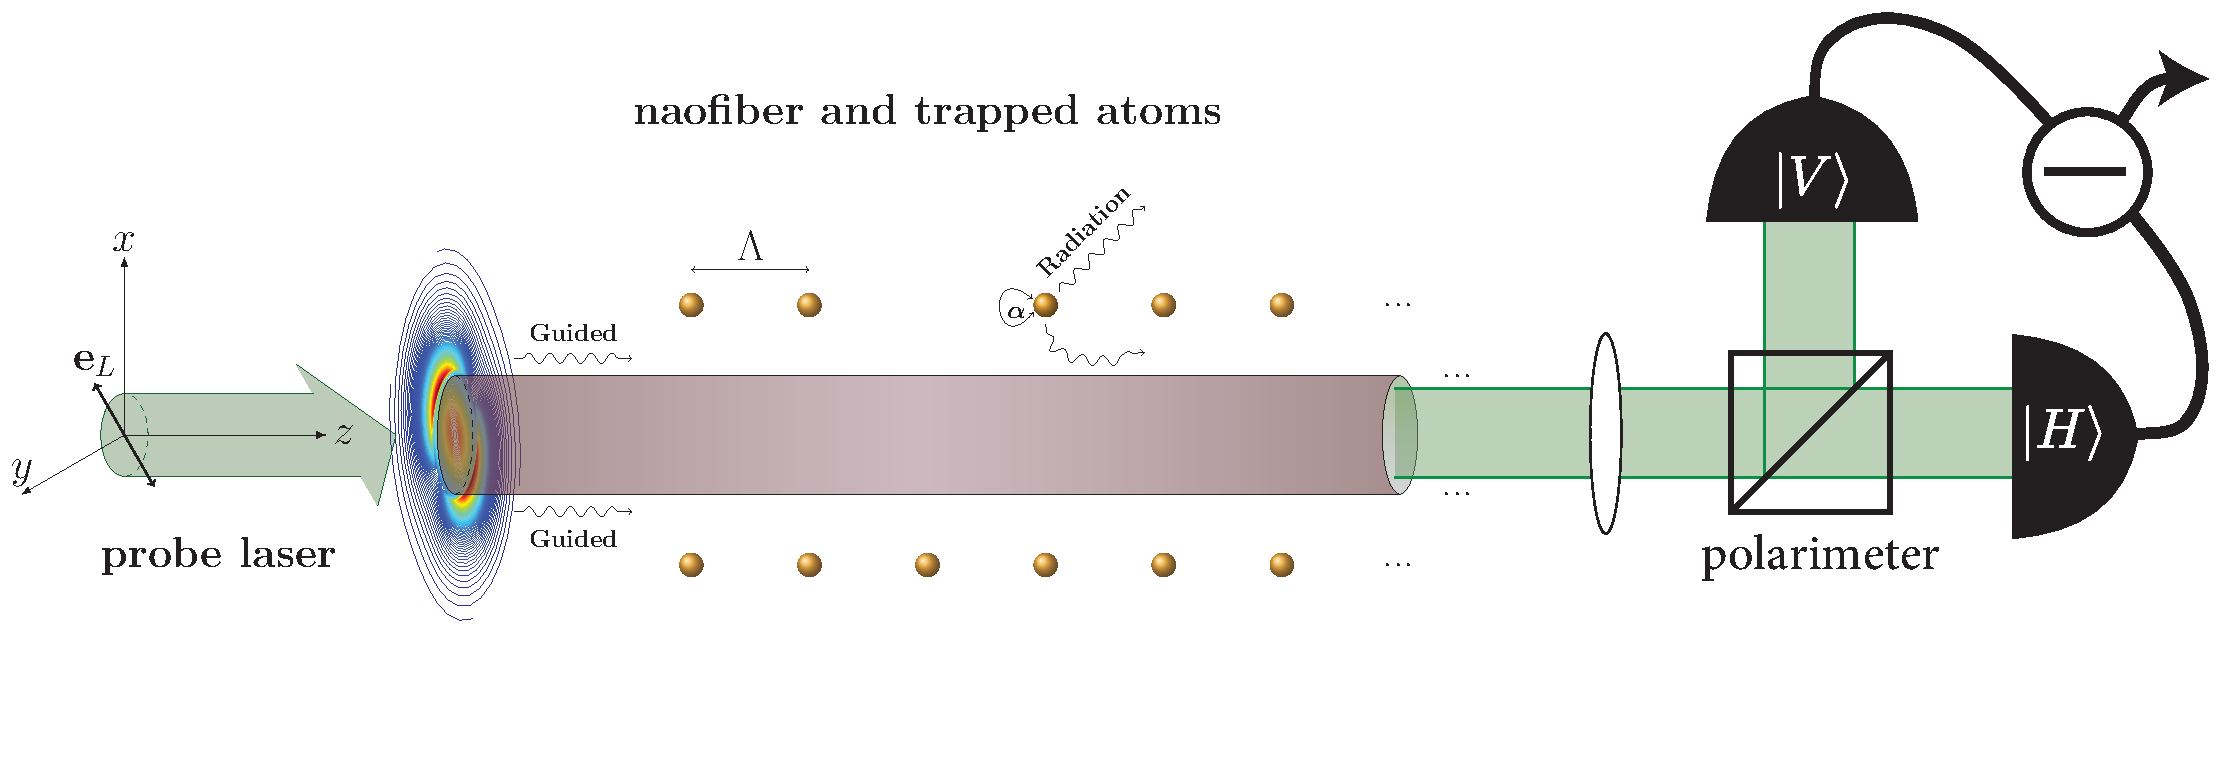
\includegraphics[scale=0.35]{./Figs/BirefringenceMeasurement_randomAtoms}
\caption{Birefringence measurement setup for a nanofiber trapped atomic system. In the evanescent 
field of the nanofiber, atoms (golden balls) randomly  occupy the periodic trapping sites on both sides of 
a 1D-chain with a period of $\Lambda$.}
\label{fig:BirefringenceMeasurement}
\end{figure}

\section{Dyadic Green's function and input-output field response}

Given a point particle at position $\br'$ with tensor polarizability $\tensor{\boldsymbol{\alpha}}$, the  
scattering solution to the wave equation at frequency $\omega_0$, 
\begin{align}\label{eq:Maxwellwithsource2}
\left[ - \nabla \times\nabla \times + n^2(\br)k_0^2 \right] \mathbf{E}(\br) &= -4\pi  k_0^2 
\delta^{(3)}(\br-\br')\;  \tensor{\boldsymbol{\alpha}}\cdot \mathbf{E}(\br),
\end{align}
is given by the Lipmann-Schwinger equation \cite{wubs_multiple-scattering_2004}
\begin{align}
\mathbf{E}_{\out}(\br) &=\mathbf{E}_{\inp}(\br)+\tensor{\mathbf{G}}^{(+)}(\br , \br'; \omega_0)\cdot 
\tensor{\boldsymbol{\alpha}}\cdot \mathbf{E}_{\out}(\br')\\
&\approx \mathbf{E}_{\inp}(\br)+ \tensor{\mathbf{G}}^{(+)}(\br , \br'; \omega_0) \cdot 
\tensor{\boldsymbol{\alpha}}\cdot \mathbf{E}_{\inp}(\br'), \label{Eq::ScatteredField}
\end{align}
where $\mathbf{E}_{\inp}(\br)$ is the asymptotic input field, $\tensor{\mathbf{G}}^{(+)}$ is the retarded (causal) Green's function solution, and in the second line we have made the first Born approximation valid for weak scattering. The fundamental object appearing in \erf{Eq::ScatteredField} that fully characterizes the scattered radiation and the modification of atomic radiation near dielectric surfaces is the dyadic Green's function, $\tensor{\mathbf{G}}(\br, \br';\omega)$, which satisfies the vector Helmholtz equation,
 \begin{align}
\left[ -\nabla\times\nabla\times + n^2(\mbf{r}) k^2 \right] \tensor{\mathbf{G}}(\br, \br';\omega) &= -4 \pi 
k^2 \delta^{(3)}(\mathbf{r}-\mathbf{r}') \tensor{\mathbf{I}},
\end{align}
where $k=\omega/c$ and $n(\mbf{r})$ is the spatially anisotropic index of refraction; Gaussian-cgs units are used throughout.  On resonance, at $\br=\br'$, 
$\Im\left(\tensor{\mathbf{G}}(\br', \br'; \omega= \omega_A) \right)$ determines the Purcell effect \cite{}.  We 
seek here the off-resonance, dispersive response.



A complete solution for $\tensor{\mathbf{G}}(\br ,\br' ; \omega_0)$ following from Maxwell's equations 
has been studied previously \cite{sakoda_optical_1996,sondergaard_general_2001}.  As we are interested here in the forward-scattered components that lead to phase shifts and polarization transformations, we directly calculate $\tensor{\mathbf{G}}(\br ,\br' ; \omega_0)$ through a decomposition into normal modes.  A complete set of eigenmodes in the presence of a dielectric are defined according to the procedure of Glauber and Lewenstein~\cite{glauber_quantum_1991}.  We define a set of functions, $\tilde{\mathbf{F}}_\fidx(\br) \equiv n(\br) \mathbf{F}_\fidx (\br)$, where $\mathbf{F}_\fidx (\br)$ is proportional to the electric field of the corresponding fiber modes and has units $1/\sqrt{V}$.  These form a complete set of transverse vector functions, as they are eigenfunctions of a Hermitian operator, 
$\tensor{\mathcal{H}}(k) = -\frac{1}{n(\br)} \nabla\times\nabla\times \frac{1}{n(\br)} + k^2 \tensor{\mathbf{I}}$ according to  $\tensor{\mathcal{H}}(k_0) \cdot \tilde{\mathbf{F}}_\fidx = \lambda_\fidx \tilde{\mathbf{F}}_\fidx$, with eigenvalues $\lambda_\fidx=k_0^2-k_\fidx^2$. The complete orthonormal modes thus satisfy,
\begin{align}
\int \mathrm{d}^3\br \, \tilde{\mathbf{F}}_\fidx^* (\br)\cdot \tilde{\mathbf{F}}_{\mu'}(\br)  &= \int \mathrm{d}^3\br \, n^2(\br) 
\mathbf{F}_\fidx^* (\br)\cdot  \mathbf{F}_{\fidx'}(\br) =\delta_{\fidx, \fidx'},\label{eq:orthutrans}
\\
\sum_\fidx \tilde{\mathbf{F}}_\fidx (\br) \tilde{\mathbf{F}}_\fidx^*(\br') &= \sum_\fidx n(\br)n(\br') 
\mathbf{F}_\fidx  (\br) \mathbf{F}_\fidx^*(\br) =\tensor{\delta}^{(T)}(\br-\br'), 
\end{align}
where $\tensor{\delta}^{(T)}(\br-\br')$ is the  delta function for transverse (divergenceless) vector 
fields.  It follows that the transverse dyadic Green's function can be decomposed as~\cite{sondergaard_general_2001}
\begin{equation}
\tensor{\mathbf{G}}(\br,\br'; \omega_0) = -4\pi \sum_{\fidx} \frac{\omega_0^2\mathbf{F}_\fidx (\br) 
\mathbf{F}^*_\fidx (\br')}{\omega_0^2-\omega_\fidx^2},
\end{equation}
where $\omega_\fidx^2 = c^2 k_\fidx^2$.  This sum separates into guided an unguided (radiation) contributions. We focus here on the guided-mode contribution to the Green's function, for details concerning the radiation modes, see Ref. \cite{sondergaard_general_2001,le_kien_spontaneous_2005, le_kien_anisotropy_2014} .

We treat here an optical nanofiber of radius $a$ with step-index profile,
	\begin{align}
		n(r_\perp) = \Bigg\{  
			\begin{array}{l l} n_1 & \quad r \leq a \\
						 n_2 & \quad r > a 
		\end{array},
	\end{align}
for a silica core ($n_1 = 1.45$) and infinite vacuum cladding ($n_2 = 1$).  For a cylindrically symmetric dielectric with index of refraction depending only on the radial coordinate, the guided modes are $\mathbf{F}_\mu (\br) = \mathbf{u}_\mu (\br_\perp) e^{i\beta z}$, \comment{units are wrong, right side should have $d\beta$?} with indices $\mu=\{n, \beta, p\}$ for guided mode $n$ with propagation constant $\beta$ and polarization $p$.  The transverse mode functions have units of $1/\sqrt{A}$ and are normalized according to $\int d^2 \mbf{r}_\perp \, n^2(r_\perp)\mathbf{u}^*_\mu (\br_\perp) \cdot \mathbf{u}_\mu (\br_\perp) = 1$ \cite{le_kien_anisotropy_2014}.  Two convenient guided-mode bases are the quasilinear and quasicircular modes~\cite{kien_field_2004}, whose $z$-components satisfy the two-dimensional Schr\"{o}dinger-like equation, $\left[\nabla_T^2 +k_0^2 n^2(r_\perp) \right] u_{\mu,z} (\br_\perp) = \beta^2 u_{\mu,z} (\br_\perp)$.  

The nanofiber supports only the lowest HE$_{11}$ guided modes at frequency $\omega_0$  \cite{Yariv}, and thus we drop the mode index $n$.  In this case there are four guided modes: two polarizations $p$ each with propagation constants $\beta = \pm \beta_0$ corresponding to forward and backward propagation.  The guided-mode contribution to the dyadic Greens function is then 
\begin{equation} \label{Eq::GreensEigenmodes}
\tensor{\mathbf{G}}_g(\br,\br'; \omega_0) = \int_{-\infty}^\infty \frac{d \beta}{2 \pi} \sum_{p} 
\frac{-4\pi\omega_0^2}{\omega_0^2-\omega^2(\beta)} \mathbf{u}_{\beta,p} (\br_\perp)\mathbf{u}^*_{\beta,p} 
(\br_{\perp}^\prime) e^{i\beta(z-z')},
\end{equation}
where $ \omega(\beta)$ is the frequency of the guided HE$_{11}$ for a given $\beta$.  The 
HE$_{11}$ mode has no cutoff; for a given $\omega$, there always exists a guided mode with propagation 
constant $\beta(\omega)$.  

For $z>z'$ ($z'>z$), the contribution of the guided modes to the retarded Green's function is found by the 
usual displacement of the pole on the positive (negative) $\beta$-axis into the upper (lower) half of 
the complex plane. Closing the contour yields
\change{
\begin{align} 
\tensor{\mathbf{G}}^{(+)}_g(\br,\br'; \omega_0) = &2\pi i \sum_{f,p}  {\rm Res}\vert_{\beta =f\beta_0} 
\left[\frac{-4\pi \omega_0^2}{2\pi (\omega_0^2-\omega^2(\beta))}\right]  \mathbf{u}_{f\beta_0, p} 
(\br\!_\perp)\mathbf{u}^*_{f\beta_0, p} (\br_{\!\perp}^\prime)e^{if \beta_0 (z-z')} \nonumber \\
%&  =  i 2\pi f \frac{\omega_0}{v_g } \sum_{p} \mathbf{u}_{f, p} (\br\!_\perp)\mathbf{u}^*_{f , p} 
%(\br_{\!\perp}^\prime) e^{if \beta_0(z-z')}\;\; {\rm for }\;  (z-z')f>0,
  = & 2\pi i \frac{\omega_0}{v_g } \sum_{f,p} f  \mathbf{u}_{f, p} (\br\!_\perp)\mathbf{u}^*_{f , p} 
(\br_{\!\perp}^\prime) e^{if\beta_0(z-z')} \Theta \big((z-z')f \big) 
\label{Eq::GreensGuided}
\end{align}
}where $f=\pm$ indicates the propagation direction and $\Theta \big((z-z')f \big)$ is the Heaviside function that enforces causality; we have suppressed the label $\beta_0$ as it is implicit in the definition of the guided modes at frequency $\omega_0$. For silica-core fibers the material dispersion is small; however, a The group velocity $v_g= d\omega/d\beta \vert_{\beta=\beta_0}$ is the group velocity.  In the second line, For \change{$z=z'$} we cannot close the contour. Instead, we expand the resonant denominator in \erf{Eq::GreensEigenmodes} with the poles moved to yield the retarded (causal) response,
\begin{equation}
\frac{1}{(\omega_0+i\epsilon)^2-\omega^2(\beta)}=\frac{1}{2 \omega(\beta)}\left[ \frac{1}{\omega_0+ i 
\epsilon - \omega(\beta)} - \frac{1}{\omega_0+ i \epsilon + \omega(\beta)} \right],
\end{equation}
 and employ the usual distribution identities \cite{sondergaard_general_2001},
\begin{equation}
\lim_{\epsilon \rightarrow 0_+} \frac{1}{\omega_0 + i \epsilon \mp 
\omega(\beta)}=\mathcal{P}\left[\frac{1}{\omega \mp \omega(\beta)} \right] + i \pi \delta (\omega_0 \mp 
\omega(\beta)).
\end{equation}
As only the positive frequency component contributes to the $\delta$-function, it follows that the imaginary 
part of the Green's function at $\br = \br'$ that determines the Purcell enhancement of spontaneous 
emission into the guided modes is
	\begin{equation}
		\Im\left[\tensor{\mathbf{G}}^{(+)}_g(\br',\br'; \omega_0) \right] = \pi \frac{\omega_0}{v_g } \sum_{f, p} 
		\mathbf{u}_{f, p} (\br_{\!\perp}^\prime)\mathbf{u}^*_{f , p} (\br_{\!\perp}^\prime).
	\end{equation}
The real part determines the energy level shift on the atom due to its proximity to the dielectric.

Equation (\ref{Eq::GreensGuided}) is the central result from which we can calculate the dispersive response.  
Consider a forward-propagating input field in the guided modes with arbitrary polarization, $\mathbf{E}_{\inp}(\br) = \mathcal{E}^{(+)}_0 \mathbf{u}_{+,\rm in}(\br_\perp) e^{i \beta_0 z}$, (\comment{this $\beta_0$ corresponds to the probe frequency, not the atomic frequency}), where $\mathcal{E}^{(+)}_0$ is the peak postive-frequency electric field amplitude, and  
	\begin{align}
		\mbf{u}_{f,\rm in}(\mbf{r}_\perp) = \sum_{p} c_{f,p} \mathbf{u}_{f,p}(\br_\perp),
	\end{align}
with $\sum_{f,p} |c_{f,p}|^2 = 1$.  Substitution of the guided-mode Green's function, \erf{Eq::GreensGuided}, into the Lippman-Schwinger equation, \erf{Eq::ScatteredField}, yields the transmitted (forward-scattered) output field, 
	\begin{equation}
		\mathbf{E}_{\out}(\br) =  \mathcal{E}^{(+)}_0 \sum_{p,p'}  \, t_{pp'} c_{+,p} \mathbf{u}_{+, p'}(\br_\perp) e^{i \beta_0 z}. 
	\end{equation}
For an atom located at $\br'$, the transmission matrix is \change{
\begin{equation} \label{Eq::PolarizationTransformation}
t_{pp'} = \delta_{p,p'} + i 2\pi k_0 n_g^2 \, \mathbf{u}^*_{+, p'}(\br'_\perp) \cdot 
\tensor{\boldsymbol{\alpha}} \cdot \mathbf{u}_{+, p}(\br'_\perp) ,
\end{equation}
where $n_g = c/v_g$ is the group index of refraction.  }The diagonal terms determine the attenuation and phase shift induced on each polarization component 
according to $t_{p p} \approx \sqrt{1-R}e^{i \delta \phi_p}$ where
	\begin{align}
		\delta \phi_p &= \frac{2 \pi k_0}{A_{\rm in}} |\mathbf{u}_{\rm in}(\mathbf{r}'_\perp)|^{2} \Re(\alpha_{pp}) , \label{Eq::PhaseShift} \\
		R &=  \frac{4 \pi k_0}{A_{\rm in}} |\mathbf{u}_{\rm in}(\mathbf{r}'_\perp)|^{2} \Im(\alpha_{pp}) , \label{Eq::Attenuation}
	\end{align}
\change{The effective mode area at the atom's position is determined from the total cycle-averaged power transported along the nanofiber, $P_{\rm in} = (v_g/4\pi) |\mathcal{E}^{(+)}|^2$, and the intensity at the atom $I_{\rm in}(\mathbf{r}') = (c/4\pi)|\mathcal{E}^{(+)}|^2|\mbf{u}_{\rm in}(\mbf{r}_\perp')|^2$, via the relation \cite{domokos_quantum_2002},
 	\begin{align} \label{Eq::AreaIn}
 		A_{\rm in} \equiv \frac{P_{\rm in}}{I_{\rm in}(\mathbf{r}')} = \frac{1}{n_g |\mathbf{u}_{\rm in}(\mathbf{r}'_\perp)|^{2}}.
	\end{align}
and the $\{p,p'\}$-element of the tensor polarizability is given by }
	\begin{align}
		\alpha_{pp'} \equiv \mathbf{u}^*_{+,p}(\br'_\perp) \cdot \tensor{\boldsymbol{\alpha}}\cdot \mathbf{u}_{+, p}(\br'_\perp). \label{Eq::ModeAreaImplicit}
	\end{align} 
The phase shift per atom is modified over free space in two ways.  The mode dispersion relation 
 $\omega(\beta)$ can lead to an enhancement due to a group velocity reduction. This factor is less 
 important for the nanofiber geometry under consideration here.  More importantly, the effective mode 
 area $A_{\rm in}$ is typically orders of magnitude smaller than for a paraxial laser beam in free space.  
 
 The off-diagonal terms in the transmission matrix correspond to polarization transformations.  For 
 example, if we take the polarizations to be the quasilinear modes~\cite{?}, which we will denote $\{ 
 \mathbf{u}_{H}, \mathbf{u}_{V}\}$, then $t_{HV} \equiv \chi_{\rm Far}$,  the rotation angle of the Faraday 
 effect.  In this basis, the phase difference $\delta  \phi_H - \delta \phi_V$ corresponds to birefringence.  
 Alternatively, analyzed in the quasicircular polarization basis, $\delta \phi_+ -\delta  \phi_-$ corresponds 
 to Faraday rotation and $t_{+-}$ to birefringence.  We will use such polarization transformations as a means to nondestructively measure the atoms and generate collective spin squeezing.

{\color{blue} How does our scattering matrix relate to that from Le Kien's results about propagation of light through an array of nanofiber-trapped atoms?  Specifically, Eq. (8) of Ref. \cite{le_kien_correlations_2008} and/or Eqs. (8-10) of Ref. \cite{le_kien_propagation_2014}?  
}

\subsection{Heisenberg-Langevin-picture solution and atomic response}
The Lippmann-Schwinger solution, \erf{Eq::ScatteredField}, determines the input-output relation for linear atomic response given by the polarizability tensor $\tensor{\alpha}$.  In this section we derive the fully quantum mechanical description of dispersive atomic response and input-output relations for the quantized guided modes.  Following Ref. \cite{le_kien_spontaneous_2005}, we use a Heisenberg-Langevin approach for one-dimensional systems.  

The positive frequency component of the quantized electric field operator decomposes into guided and radiation (unguided) modes, $\hat{\mathbf{E}}^{(+)}=\hat{\mathbf{E}}_g^{(+)}+\hat{\mathbf{E}}_{r}^{(+)}$, where
\begin{align}
\hat{\mathbf{E}}_g^{(+)}(\br) &= \sum_{f,p} \int \mathrm{d}\omega \sqrt{\frac{ \hbar \omega}{v_g}} 
\hat{a}_\mu \mathbf{u}_\mu (\br\!_\perp) \change{  e^{if\beta_0 z} },\label{Eq::QuantizedElectricField} \\
\hat{\mathbf{E}}_r^{(+)}(\br) &= \sum_{m,p} \int \mathrm{d}\omega  \, \int_{-kn_2}^{kn_2}\mathrm{d}\beta \, 
\sqrt{ \hbar \omega} \hat{a}_\nu \mathbf{u}_\nu (\br\!_\perp) \change{ e^{i\beta(\omega) z} },
\end{align}
The four HE$_{11}$ guided modes are indexed by $\mu =(\omega, f, p)$ for two polarizations $p$ and two propagation directions $f=\pm1$ with wavenumbers $f\beta (\omega)$.  The radiation modes are indexed by \change{ $\nu=(\omega, \beta, m, p)$ where $\omega$ indexes the frequency, $\beta$ the longitudinal propagation constant, $m$ the azimuthal quantum number (angular momentum), and $p$ the two orthogonal polarizations} \cite{sondergaard_general_2001}.  The creation/annihilation operators satisfy the usual continuous-mode commutation relations, $[\hat{a}_\mu, \hat{a}^\dag_{\mu'} ] = \delta_{f,f'} \delta_{p,p'} 
\delta ( \omega - \omega ') $, $[\hat{a}_\nu ,\hat{a}^\dag_{\nu'} ] = \delta_{m,m'} \delta_{p,p'} \delta ( 
\omega - \omega ')  \delta ( \beta - \beta') $.

The Hamiltonian for the system is
\begin{equation}
\hat{H} = \hat{H}_F+\hat{H}_A + \hat{H}_{\inter}.
\end{equation}
The free field Hamiltonian decomposes into guided and unguided modes, 
\begin{equation}
\hat{H}_0 = \sum_{f,p}\int \mathrm{d}\omega \, \hbar \omega \hat{a}^\dagger_\mu \hat{a}_\mu 
+\sum_{m,p} \int \mathrm{d}\omega  \int_{-nk_0}^{nk_0} \mathrm{d}\beta \, \hbar \omega 
\hat{a}^\dagger_\nu \hat{a}_\nu.
\end{equation}
We consider here alkali atoms with hyperfine multiplets of ground and excited levels, $\{ 
\ket{g}=\ket{nS_{1/2}, F, M_F}\}$, $\{ \ket{e} =\ket{nP_{J'}, F', M_{F'}}\}$,
\begin{equation}
\hat{H}_A  = \sum_g E_g \ket{g}\bra{g} + \sum_e E_e \ket{e}\bra{e}.
\end{equation}
In the rotating wave approximation, the atom-field interaction Hamiltonian is
\begin{align}
\hat{H}_{\inter} &= -\hat{\mathbf{d}}\cdot \hat{\mathbf{E}} = -\hat{\mathbf{d}}_{eg}\cdot 
\hat{\mathbf{E}}^{(+)}(\br')-\hat{\mathbf{d}}_{ge}\cdot \hat{\mathbf{E}}^{(-)}(\br'),
\end{align}
where the atomic dipole operator is projected between excited and ground subspaces, $\hat{\mathbf{d}}_{eg}= \hat{P}_e \hat{\mathbf{d}} \hat{P}_g $. The interaction Hamiltonian then takes the form, 
\begin{equation}
\hat{H}_{\inter} = -\sum_{g,e} \left(\sum_{f,p} \int\mathrm{d}\omega \; \hbar g_{\mu, e,g}\, \hat{a}_\mu  \, 
\hat{\sigma}_{eg}+ \sum_{m,p} \int\mathrm{d}\omega \! \int_{-kn_2}^{kn_2}\mathrm{d}\beta \,  \hbar 
g_{\nu, e,g}\, \hat{a}_\nu \, \hat{\sigma}_{eg}+  h.c.\right),
\end{equation}
where $\hat{\sigma}_{\alpha\beta}= \ket{\alpha}\bra{\beta}$ are the two-level atomic lowering operators, and 
the coupling constants between the electric dipole and the guided/radiation modes are
\begin{subequations} \label{Eq::CouplingConstants}
\begin{align}
\hbar g_{\mu, e,g} &= \sqrt{\frac{\hbar \omega}{v_g}}\; \bra{e} \hat{\mathbf{d}} \ket{g} 
\cdot\mathbf{u}_\mu (\br') \change{  e^{i f \beta_0z} }, \\
\hbar g_{\nu, e,g} &= \sqrt{\hbar \omega} \; \bra{e} \hat{\mathbf{d}} \ket{g} \cdot \mathbf{u}_\nu (\br')  \change{  e^{i\beta(\omega)z} } .
\end{align}
\end{subequations}
The Heisenberg equations of motion thus follow,
\begin{align}
\der{\hat{a}_\mu} &= -i\omega \hat{a}_\mu +i\sum_{e,g} g_{\mu, e,g}^* \hat{\sigma}_{ge} \label{eq:da}\\
\der{\hat{a}_\nu} &= -i\omega \hat{a}_\nu +i\sum_{e,g} g_{\nu, e,g}^*  \hat{\sigma}_{ge} \label{eq:danu}\\
\der{\hat{\sigma}_{ge}} &= -i\omega_{eg} \hat{\sigma}_{ge} \nonumber\\
&+ i\int_0^{\infty}\mathrm{d}\omega \sum_{e',g'} \bigg[ \big(\delta_{ee'} \hat{\sigma}_{gg'} - \delta_{gg'} 
\hat{\sigma}_{e'e} \big) \bigg\{ \sum_{f,p}  g_{\mu, e',g'}\hat{a}_\mu +\sum_{m,p}  
\int_{-kn_2}^{kn_2}\mathrm{d}\beta \; g_{\nu, e',g'} \hat{a}_\nu \bigg\} \bigg] \label{Eq::dsigma} 
\end{align}
Integrating the field equations, 
\begin{subequations}\label{eq:aout1}
\begin{align}
\hat{a}_\mu(t) &= \hat{a}_\mu(t_0) e^{-i\omega (t-t_0)} +i \sum_{e,g} g_{\mu,e,g}^* \int_{t_0}^t 
\mathrm{d} t' e^{-i\omega (t-t')}\hat{\sigma}_{ge}(t') \label{Eq::aguidedEOM}
\end{align}
\begin{align}
\hat{a}_\nu (t) &= \hat{a}_\nu (t_0) e^{-i\omega (t-t_0)} +i \sum_{e,g} g_{\nu,e,g}^* \int_{t_0}^t \mathrm{d} 
t' e^{-i\omega (t-t')}\hat{\sigma}_{ge}(t'),
\end{align}
\end{subequations}
\comment{how to properly label the modes here vs. the propagating modes later?} and substituting into \erf{Eq::dsigma}, and making the standard Markov approximation~\cite{?} yields
\begin{align}
&\dt{\hat{\sigma}_{ge}} =-i\omega_{eg} 
\hat{\sigma}_{ge}-\sum_{e'}\frac{\Gamma_{ee'}}{2}\hat{\sigma}_{ge'}  \\
&+i \sum_{e'g'}\bigg[ (\delta_{e,e'} \hat{\sigma}_{gg'} - \delta_{g,g'} 
\hat{\sigma}_{e'e})\int_0^{\infty}\mathrm{d}\omega \bigg\{\sum_{f,p}  g_{\mu, e',g'}\; \hat{a}_\mu (t_0) 
+\sum_{m,p}  \int_{-kn_2}^{kn_2}\mathrm{d}\beta \; g_{\nu, e',g'} \;\hat{a}_\nu(t_0) \bigg\} e^{-i\omega 
(t-t_0)}\bigg] \nonumber
\end{align}
where the decay of excited state correlations is given by 
\begin{equation}
\Gamma_{ee'} = 2\pi \sum_{f,p,g} g_{\mu,e,g}g^*_{\mu,e',g} \vert_{\omega=\omega_{eg}}+2\pi 
\sum_{m,p,g'} \change{ \int d\beta } \, g_{\nu,e,g}g^*_{\nu,e',g'} \vert_{\omega=\omega_{eg}},\label{Eq::TotaleeDecayRate}
\end{equation}
\change{and the small Lamb shifts are absorbed into the transition frequency $\omega_{eg}$.} 

The first sum describes decay into the guided modes and the second into the unguided radiation 
modes \cite{domokos_quantum_2002, klimov_spontaneous_2004,le_kien_spontaneous_2005}.  Thus, the total spontaneous emission rate of a given excited state into the guided modes is
\begin{equation}
\Gamma_e^{\oneD}= 2\pi \sum_{f,p,g} \big|g_{\mu,e,g} \big|^2_{\omega = \omega_{eg}} =  \sum_{f,p,g}\frac{2 \pi \big|\bra{e}\hat{\mathbf{d}}\ket{g} \cdot \mathbf{u}_{fp}(\br'_\perp)\big|^2}{\hbar} 
\left(\frac{\omega_{eg}}{v_g}\right).
\end{equation}
This agrees with the expected expression~\cite{?} following from the guided-mode contribution to the 
dyadic Green's function, \erf{Eq::GreensGuided},
\begin{equation}
\Gamma_e^{\oneD} = \sum_{g}   \frac{2}{\hbar} \; \bra{g}\hat{\mathbf{d}}\ket{e}\cdot 
\Im\left(\tensor{\mathbf{G}}^{(+)}_g(\br', \br'; \omega= \omega_A) \right) \cdot 
\bra{e}\hat{\mathbf{d}}\ket{g},
\end{equation}
enhanced over the free space rate by the Purcell factor.  \comment{We really should include a small plot of $\Gamma_{\rm 1D}/\Gamma_0$ for some chosen parameters.  For those outside of the nanofiber community, this is the \emph{first} thing they ask.  The point is that while it's not so high, it's still quite small, and we can  benefit from many atoms much more easily than those alligator waveguide photonic crystals.}

Here we are interested in linear response for excitation far from resonance.  In steady state, the dipole 
operator in the linear regime ($\hat{\sigma}_{ee'} \rightarrow 0 $) is approximately
\begin{align}
\hat{\sigma}_{ge} \approx -\sum_{g'} \hat{\sigma}_{gg'}\int_0^{\infty}\mathrm{d}\omega \bigg( & \sum_{f,p}  
\frac{g_{\mu, e,g'}}{\omega-\omega_{eg} \error{- i \Gamma_{e}/2 } }\, \hat{a}_\mu (t_0) \\
	&+\sum_{m,p} \int_{-kn_2}^{kn_2}\mathrm{d}\beta \, \frac{g_{\nu, e,g'}}{\omega-\omega_{eg}\error{- i \Gamma_{e}/2 }} \,\hat{a}_\nu (t_0)  \bigg)e^{-i\omega (t-t_0)} , \nn
\end{align}
where $\Gamma_e$ is the total decay rate from excited state $\ket{e}$, given by the diagonal elements of \erf{Eq::TotaleeDecayRate}.  By substituting this into \erf{Eq::aguidedEOM} and defining asymptotic modes, \comment{ $\hat{a}^{\inp}(\omega) = \lim_{t_0\rightarrow -\infty} \hat{a}(t_0) e^{i\omega t_0}$, $\hat{a}^{\out}(\omega) = \lim_{t\rightarrow +\infty} \hat{a}(t) e^{i\omega t}$ \cite{fan_input-output_2010} }, we obtain the input-output relationships of the guided modes due to the presence of an atom close to the nanofiber,
\begin{equation}
\hat{a}^{\out}_\mu (\omega) = \hat{a}^{\inp}_\mu (\omega) \!-\! i\sum_{p',f'} 
\sum_{e,g,g'}\!\hat{\sigma}_{gg'}\frac{2\pi g_{\mu,e,g}^* 
g_{\mu',e,g'}}{ \Delta_{eg} -  \error{i \Gamma_{e}/2 }}\hat{a}^{\inp}_{\mu'}(\omega) \!-\! i\sum_{m,p} 
\sum_{e,g,g'}\!\hat{\sigma}_{gg'}\frac{2\pi  g_{\mu,e,g}^* 
g_{\nu',e,g'}}{ \Delta_{eg} \error{ - i \Gamma_{e}/2 }}\hat{a}^{\inp}_{\nu}(\omega).
\end{equation}
This agrees with the expected form given by the Lippmann-Schwinger equation in the first Born 
approximation,
\begin{equation} \label{Eq::IOScatteredField}
\hat{\mathbf{E}}^{(+)}_{g,\out}(\br)=\hat{\mathbf{E}}^{(+)}_{g, 
\inp}(\br)+\tensor{\mathbf{G}}_g^{(+)}(\br,\br',\omega)\cdot \poltens \cdot 
\left(\hat{\mathbf{E}}^{(+)}_{g, \inp}(\br')+\hat{\mathbf{E}}^{(+)}_{r, \inp}(\br')\right),
\end{equation}
by noting
\comment{
\begin{equation}
\mathbf{u}^*_{\mu} (\br)\cdot \tensor{\mathbf{G}}_g^{(+)}(\br,\br',\omega)\cdot 
\poltens \cdot \mathbf{u}_{\mu'} (\br') = i 2\pi k\frac{c}{v_g} \mathbf{u}^*_\mu 
 (\br) \cdot \poltens \cdot \mathbf{u}_{\mu'} (\br') = - i \sum_{e,g,g'}\!\ 
 \hat{\sigma}_{gg'} \frac{2\pi g_{\mu,e,g}^* g_{\mu',e,g'}}{\change{ \Delta_{eg} - i \Gamma_{e}/2 }}, 
\end{equation}
 Don't we need a projection integral to make Eq. (38) correct?  Then, is it strictly correct? What about backward modes? The $\mbf{u}(\mbf{r}_\perp)$ functions are only labeled by the transverse spatial components.} where the guided-mode dyadic Green's function is given in \erf{Eq::GreensGuided} and the atomic polarizability tensor operator is
\begin{equation} \label{Eq::PolarizabilityOperator}
\poltens = - \frac{1}{\hbar} \sum_{e,g,g'}\ket{g'}\frac{\bra{g'}\hat{\mathbf{d}}\ket{e}\bra{e} 
\hat{\mathbf{d}}\ket{g}}{\Delta_{eg}  \error{- i \Gamma_{e}/2 }}\bra{g}.
\end{equation}
Scattering of classical waves follows when the field is in a coherent state.  The phase-shift on a guided mode with a given polarization $p$, \erf{Eq::PhaseShift}, now depends on the internal state of the atom.  Given atoms in a particular ground sublevel $\ket{g}$, this can be expressed \cite{le_kien_propagation_2014}
\begin{equation} \label{Eq::PhaseShiftMultilevel}
\delta  \phi_{p,g} =2\pi k_0 \frac{c}{v_g}\mathbf{u}^*_{+, p}(\br'_\perp) \cdot \bra{g} 
\hat{\tensor{\boldsymbol{\alpha}}} \ket{g} \cdot \mathbf{u}_{+, p}(\br'_\perp) = -\frac{1}{\hbar} \sum_e \frac{2 \pi 
|\bra{e}\hat{\mathbf{d}}\ket{g} \cdot \mathbf{u}_{+,p}(\br'_\perp)|^2}{   \Delta_{eg} - \error{i \Gamma_{e}/2 }} 
\left(\frac{ \change{ \omega_{eg}} }{v_g}\right).
\end{equation}
\comment{ Should we include here the full polarization transformation $S$-matrix akin to \erf{Eq::PolarizationTransformation}?}  For weak excitation due to large detuning, $\Gamma_{e}/\Delta_{eg} \ll 1$ and the scattering is entirely elastic.  In this case, the absorption loss can be ignored and \erf{Eq::PhaseShiftMultilevel} describes a pure dispersive phase shift.


In relation to \erf{Eq::phaseshift} we see that $\delta \phi \propto (\sigma_0/\tilde{A}) (\Gamma_{\oneD}/\Delta)$, where $\sigma_0$ is the resonant scattering cross section, and $\tilde{A}$ is the effective mode area defined in \erf{Eq::ModeAreaImplicit}. \comment{Again, the mode area is only implicitly defined there.  We need to be clearer about it.}  For comparison, the phase shift on a paraxial laser beam imparted by an atom in vacuum  has the same form as \erf{Eq::PhaseShiftMultilevel}, but with the guided mode replaced by the $\mathrm{TEM}_{00}$ mode of a laser field at the atom position, with area $A= \pi w_0^2/2$ and beam waist $w_0$ \cite{tanji-suzuki_chapter_2011,baragiola_three-dimensional_2014}. The strongest phase shift in free space is achieved when the atom is placed at the center of the beam waist where the intensity is largest. The relative strength of the phase shift is $\delta \phi_{\rm fiber}/\delta \phi_{\vac}\propto (A/\tilde{A}) (c/v_g)$, as plotted in Fig. ? as a function of the radial position of the atom \comment{(paraxial beam waist on the other axis (contour plot), and what about choice of atomic state?  Le Kien's recent paper only considered mixed states; specifically an equal distribution of population among the sublevels for which there was no polarization transformation, only phase shifts)}.  For example, for a quasilinear field, and an atom trapped along the direction of the input polarization  at $r_\perp = ?$, $\delta \phi_{\rm fiber}/\delta \phi_{\vac} = ?$.   Thus we see that, in the nanofiber geometry the Purcell factor does not cause the majority of scattering to be guided, nor is the phase shift enhanced greatly over the phase shift imparted by an atom at the center of a paraxial beam. However, the key feature is that for a chain of atoms trapped along the fiber, the phase shifts add linearly.  Thus, one can achieve an effective optical density in the fiber geometry with far fewer atoms ($\sim 1000$ atoms) than would be required in free space (\error{ $\sim 10^6$ }).  The result is a much larger average entangling interaction \emph{per atom} whose application in QND measurement we explore in the following section.

\missingfigure{Figure for the enhancement comparison.}


\section{QND measurement of atoms}
The dispersive interaction between the atoms and nanofiber guided photons provides a mechanism with which to perform a QND measurement on the atoms.  We take the atoms to be trapped along the $x$-axis at position $(r'_\perp =a, \phi' =0)$.  We restrict here to two quasi-linear polarizations, $p =\{H,V\}$, of the single HE$_{11}$ guided mode \comment{ propagating in the positive $z$-direction ($f = +$) }.  Outside the fiber, the transverse mode functions are~\cite{tong_single-mode_2004,kien_field_2004}
\comment{
\begin{subequations} \label{Eq::NanofiberModes}
\begin{align}
u_{H,x}(r_\perp,\phi) &= u_0 \frac{\beta_0}{2 q}[(1-s)K_0(q r_\perp) - (1+s)K_2(q r_\perp) \cos(2 \phi)], \\
u_{H,y}(r_\perp,\phi) &=-u_0 \frac{\beta_0}{2 h}  (1+s)K_2(q r_\perp) \sin(2 \phi) ,\\
u_{H,z}(r_\perp,\phi) &=iu_0 \frac{J_1(ha)}{K_1{qa}} K_1(q r_\perp) \cos(\phi), \\
u_{V,x}(r_\perp,\phi) &= u_0 \frac{\beta_0}{2 q}(1+s)K_2(q r_\perp) \sin(2 \phi)] ,\\
u_{V,y}(r_\perp,\phi) &=u_0 \frac{\beta_0}{2 h} [(1-s)K_0(q r_\perp) - (1+s)K_2(q r_\perp) \cos(2 \phi)], \\
u_{V,z}(r_\perp,\phi) &=iu_0 \frac{J_1(ha)}{K_1{qa}}K_1(q r_\perp) \sin(\phi), 
\end{align}
\end{subequations}
}
where $u_0$ is set by the normalization condition, $\int d^2 r_\perp n(r_\perp) | \mathbf{u}_\mu(\br_\perp)|^2=1$, $J_n$ and $K_n$ are Bessel functions of the first and second kind, $h=\sqrt{n^2 k_0^2 - \beta_0^2}$, $q=\sqrt{\beta_0^2- k_0^2}$, and $s = [(q a)^{-2} + (h a)^{-2}]/[J'_1(ha)/haJ_1(ha) + K'_1(qa)/qaK_1(qa)]$.  \comment{ I think we should include $f$ up until the Eq. (49).  The hope is that others can not only use our results, but also take advantage of all the work we've done understanding this problem.  Otherwise, why did we even include $f$ above?  Maybe we should put these functional forms in an appendix and use the somewhat simpler notation of Le Kien in the main text.  At some point we should write down the functional forms for the atom on the $x$-axis, since we use them in the numerics and they're relatively simple.  Further, it is evident how the out-of-phase $z$-component comes in to play.  We should include a little more detail about the fiber modes themselves, not necessarily equations, but expalantions.}  \change{The quasilinear fiber modes, $\mathbf{u}_H$ and $\mathbf{u}_V$, adiabatically connect through the fiber taper to $x$- and $y$-linearly polarized plane-wave modes.  We see from Eqs. (\ref{Eq::NanofiberModes}) that in the nanofiber region that $\mathbf{u}_H$ is purely $x$-polarized at $\phi = \pi/2$ and the  $\mathbf{u}_V$ is purely $y$-polarized at $\phi = 0$.  At all other azimuthal angles the electric field is generally rotating along an ellipse. }  

The Lippmann-Schwinger scattering equation, \erf{Eq::IOScatteredField}, follows in the time domain as the evolution of \error{coarse-grained} input-ouput modes \cite{gardiner_input_1985, fan_input-output_2010}.  For each HE$_{11}$ guided mode we define propagating continuous-mode annihilation operators~\cite{blow_continuum_1990, le_kien_correlations_2008},
\begin{align}
%\hat{a}_\mu(z,t) = \int \frac{d \omega}{\sqrt{2 \pi}} \; \hat{a}_\mu e^{i(n_\mu(\omega) kz-\omega t)} \\
\hat{a}_{f,p}(z,t) = \int \frac{d \omega}{\sqrt{2 \pi}} \; \hat{a}_{f,p} e^{i[\beta(\omega)z-\omega t ]} \\
	 \change{ = \int \frac{d \omega}{\sqrt{2 \pi}} \, \hat{a}_{f,p} e^{i f \beta_0( z-v_p t)}, }
\end{align}
\comment{ should the exponent be $\beta(\omega)$ or $\beta_0$?}
that satisfy the free-field commutation relations,
\change{
\begin{equation}
\big[\hat{a}_{f,p}(z,t),\hat{a}^\dag_{f',p'}(z',t')\big]=\delta_{f,f'}\delta_{p,p'}  \delta(t-t'-(z-z')/\error{v_g}).
\end{equation}
}
\comment{The phase velocity, $v_p = \omega/\beta$, directly appears in the exponential; see Refs. \cite{le_kien_correlations_2008} and \cite{le_kien_propagation_2014}. Side note: Le Kien states below Eq. (9) of Ref. \cite{le_kien_propagation_2014} that the group and phase velocities are evaluated at the \emph{laser}, not the transition, frequency}.  

We now focus on the forward-scattered modes $(f=+)$ and drop the $f$ index. The quantized electric field operator, \erf{Eq::QuantizedElectricField}, for these guided modes is
\begin{equation}
\hat{\mathbf{E}}^{(+)}(r\!_\perp,\phi,z;t) = \sqrt{ \frac{2 \pi \hbar \omega_0}{ v_g} } \Big[ \mathbf{u}_H(r\!_\perp,\phi) \hat{a}_H(z,t) + \mathbf{u}_V(r\!_\perp,\phi) \hat{a}_V(z,t) \Big] e^{i \beta_0 z},
\end{equation}
whose interaction with atoms in the dispersive regime is governed by  light-shift Hamiltonian~\cite{deutsch_quantum_2010,kien_dynamical_2013}
\begin{equation}  
	\hat{H}_{LS}   = - \sum_i \hat{\mathbf{E}}^{(-)}(\mathbf{r}'_i ; t ) \cdot \poltens\phantom{}^{(i)} \cdot \hat{\mathbf{E}}^{(+)}(\mathbf{r}'_i;t ).
\end{equation}
Here $\poltens\phantom{}^{(i)}$ is the polarizability tensor operator, \erf{Eq::PolarizabilityOperator}, for the $i^{th}$ atom trapped near the nanofiber surface at position $\mathbf{r}'_i$. The Hamiltonian thus takes the form,
\begin{align}  
	\hat{H}_{LS}   & {\color{blue} = -\frac{2 \pi \hbar \omega_0}{v_g} \sum_i \sum_{p,p'} \hat{\alpha}_{p p'}\, \hat{a}_{p}^\dag(z_i,t)  \hat{a}_{p'}(z_i,t) } \\
	& = -\frac{2 \pi \hbar \omega_0}{v_g} \sum_i   \big[\hat{\alpha}_{HH}+\hat{\alpha}_{VV} \big]_i \hat{S}_0(z_i,t) +  \big[\hat{\alpha}_{HH}-\hat{\alpha}_{VV} \big]_i \hat{S}_1(z_i,t) \label{Eq::GenHamiltonian} \\
	&\quad \quad \quad \quad \quad \quad+ \big[\hat{\alpha}_{HV}+\hat{\alpha}_{HV} \big]_i \hat{S}_2(z_i,t) + i  \big[\hat{\alpha}_{HV}-\hat{\alpha}_{VH} \big]_i \hat{S}_3(z_i,t)  \nonumber
	\end{align}
\comment{should we ignore the propagation time here; $\hat{S}_3(z_i,t) \rightarrow \hat{S}_3(t)$?  Also, superscript ${[]}^{(i)}$ for the polarizability operators?  Would there ever be a case where the spatial modes at the atoms could be different?}  where the $\{H,V\}$-components of the polarizability tensor operator are
\begin{equation}  
	\hat{\alpha}_{p p'}^{(i)}= \mathbf{u}^*_p(r'_{\perp i},\phi'_i)  \cdot \poltens\phantom{}^\error{(i)} \cdot \mathbf{u}_{p'}(r'_{\perp i},\phi'_i),
\end{equation}
\error{(just realized that the superscript inside parentheses is how we denote the irreducible components of the polarizability.  We need to think on notation.)} and
\begin{align}
\hat{S}_1(z,t) = \frac{1}{2}\left(\hat{a}^\dag_H \hat{a}_H-\hat{a}^\dag_V \hat{a}_V \right), \; \hat{S}_2(z,t) = \frac{1}{2}\left(\hat{a}^\dag_H \hat{a}_V+\hat{a}^\dag_V \hat{a}_H \right), \; \hat{S}_3(z,t) = \frac{1}{2i}\left(\hat{a}^\dag_H \hat{a}_V-\hat{a}^\dag_V \hat{a}_H \right) 
\end{align}
\comment{ do we need to label $\hat{a}_H \rightarrow \hat{a}_H(z,t)$? if not, we have skipped a notational step.} are the propagating components of the vector Stokes operator for the photon flux, which satisfy equal-$z$ commutation relations
\begin{equation}
\big[\hat{S}_i(z,t), \hat{S}_j(z,t')\big] =i \epsilon_{ijk} \delta(t-t')  \hat{S}_k(z,t).
\end{equation}
Finally, the total photon flux in the forward-propagating guided modes is given by
\begin{equation}
\hat{S}_0(z,t) = \frac{1}{2}\left(\hat{a}^\dag_H \hat{a}_H+\hat{a}^\dag_V \hat{a}_V \right).
\end{equation}

We explore a QND measurement of cesium atoms in the hyperfine manifold of the electronic ground state, $6S_{1/2}$, via polarization spectroscopy.  The polarizability tensor decomposes into irreducible components depending on detuning near the D1- or D2-resonance ($6P_{J'}$),
\comment{
\begin{align}
\hat{\alpha}_{ij} &= \sum_{F,F'} \hat{\alpha}_{ij}^{(0)}(F',F)+\hat{\alpha}_{ij}^{(1)}(F',F)+\hat{\alpha}_{ij}^{(2)}(F',F)\\
&=\sum_{F,F'} \change{\charpol} \left[ C_{J'FF'}^{(0)} \delta_{ij}+ iC_{J'FF'}^{(1)}\epsilon_{ijk}\hat{F}_k+ C_{J'FF'}^{(2)}\left(\smallfrac{1}{2} ( \hat{F}_i\hat{F}_j +\hat{F}_j\hat{F}_i )-\smallfrac{1}{3}\hat{\mathbf{F}}^2 \delta_{ij} \right) \right], \label{Eq::PolarizabilityIrrep}
\end{align}
This notation is confusing, since Eq. (54) uses subscripts to indicate $HV$ modes, contains the spatial information about the modes as well as their dimensions, and here the subscripts are used to indicate Cartesian components.} where $\hat{\mathbf{F}}$ is the hyperfine spin operator, $\change{\charpol} = -(\sigma_0/8\pi k_0) (\Gamma/\Delta_{F'F})$ is the characteristic dynamic polarizability for a resonant scattering cross section $\sigma_0 = 3 \lambda^2/2\pi$, and $C_{J'FF'}^{(K)}$ are the tensor expansion coefficients~\cite{deutsch_quantum_2010}.  \change{ To distinguish collective from single-atom operators, I recommend using lowercase $\hat{\mbf{f}}$ here.  Also, $\mbf{F}$ is used previously for the complete set of mode functions.}  The atomic polarizability tensor describes the atom's nonlinear response to an applied field, which results in polarization- and state-dependent phase shifts [\erf{Eq::PhaseShiftMultilevel}].  The nanofiber geometry also gives rise to unique features of polarization spectroscopy not present in free space.  The spatial anisotropy of the intensity for the quasilinearly polarized guided modes leads to unequal scattering of the $H$ and $V$ modes, giving rise to intrinsic birefringence, even for a purely scalar atomic polarizability.  In particular, choosing the quasi-$H$ axis along the radial direction of the trapped atom leads to a phase delay of this mode relative the fast quasi-$V$ axis.  \change{ Do we need to explain why these are \emph{quasi}-axes?  It might not be evident to anyone but the experts.  We should just define what they are- in figure, even.} This birefringence was exploited by Dawkins {\em et al.}~\cite{dawkins_dispersive_2011} as mechanism for implementing a dispersive QND measurement of the number of atoms trapped around the nanofiber, as we treat here.

Consider $N_A$ atoms, each in a completely mixed state.  \change{ In that case the $\langle \hat{\alpha}_{ij} \rangle = \sum_{F,F'} \charpol C_{J'FF'}^{(0)} \delta_{ij}$.  With atoms trapped along the quasi-$H$ axis, $\langle \hat{\alpha}_{HV} \rangle = \langle \hat{\alpha}_{HV} \rangle =0$, but  $\langle \hat{\alpha}_{HH} \rangle \neq  \langle \hat{\alpha}_{VV} \rangle$. } The resulting Hamiltonian, \erf{Eq::GenHamiltonian}, takes the form
\begin{align}
%\hat{H} = -2\pi \hbar  {\color{red}n_g} k_0 N_A \left(\hat{\alpha}_{HH}  - \hat{\alpha}_{VV}\right) =\hbar \chi N_A {\color{blue} \hat{S}_1(0,t) },
\hat{H}_{LS} &= \change{-2\pi \hbar  \comment{n_g} k_0 \sum_i \left(\hat{\alpha}^{(i)}_{HH}  - \hat{\alpha}^{(i)}_{VV}\right)\hat{S}_1(z_i,t) } \\
	& \change{\approx \hbar \chi N_A \comment{ \hat{S}_1(t) } }, \label{Eq::MixedHamiltonian}
\end{align}
\comment{ this is the first place where the group index $n_g$ appears. What benefit is there to using it?  we need to define it somewhere.  Also, we should justify using $\hat{S}(z_i,t) \rightarrow \hat{S}(0,t) = \hat{S}(t) $ for all atoms; I don't think that is done in Le Kien's paper.}  where we have excluded the coupling to $\hat{S}_0$, which plays no role in the polarization spectroscopy, and have neglected the retardation associated with the different positions of the atoms along $z$.  \change{For atoms in a completely mixed state, the rank-2 terms in the atomic polarizability, \erf{Eq::PolarizabilityIrrep}, vanish, and the rotation angle on the Poincar\'{e} sphere is determined entirely by rank-0 the scalar terms}
\begin{equation} \label{Eq::RotationAngle}
\chi = \error{-}n_g  \frac{\sigma_0}{\tilde{A}}  \sum_{F,F'}  C_{J'FF'}^{(0)} \frac{\Gamma}{4 \Delta_{F'F}}.
\end{equation}
Here, we define $\tilde{A}^{-1} \equiv |\mathbf{u}_{H}(\br'_\perp)|^2 - |\mathbf{u}_{V}(\br'_\perp)| ^2 $ as the effective area characterizing the birefringence coupling constant. \comment{ This effective area would be different for a non-mixed state and would depend on all sorts of atomic expectation values.  For arbitrary classical input fields, the effective mode area in the dominant terms will depend on the expansion coefficients.  Again, I think we should find a way to choose a characteristic area.} The effective optical density per atom is $\sigma_0/\tilde{A}$.  {\color{red}  Give some characteristic numbers.}  

\change{Dawkins {\em et al.} To use this interaction for a QND measurement of $N_A$, launched linearly polarized light at 45$^\circ$ to the quasi-$H$ axis; i.e. along the $S_2$-axis.  The input Stokes vector, $\langle \hat{S}_2^{\rm in}(t)\rangle  = \dot{N}_L/2$ for photon flux $\dot{N}_L$, rotates around the $S_1$-axis on the Poincar\'{e} sphere via to the Hamiltonian, \erf{Eq::MixedHamiltonian}.  For short times when photon scattering can be neglected, the $S_3$-component evolves according to the input-output relation,
\change{
\begin{equation}
\hat{S}_3^{\rm out}(t) = \hat{S}_3^{\rm in}(t) + \chi N_A \hat{S}_2^{\rm in}(t).
\end{equation}
}
\comment{Here, it is a little confusing that the operators on the right side have the superscript ``in."  These are the operators that appear in the Hamiltonian above, and perhaps should have no labels at all?  Or we should make sure we're clear about what they mean.  These are \emph{different} from the ``in" and ``out" operators in the Heisenberg-Langevin section; specifically, they are the Fourier transforms.  } Thus, the polarization rotation is detected by measuring the $S_3$-Stokes component, integrated over time, as described by the measurement operator,
	\begin{align}
		\hat{\mathcal{M}} &= \int_0^t dt' \hat{S}_3^{\rm out}(t) = \int_0^t dt' \big(\hat{S}_3^{\rm in}(t') + \chi N_A \hat{S}_2^{\rm in}(t') \big),
	\end{align}
with contributions from shotnoise, $\Delta \mathcal{M}_{\rm SN}^2$, and atomic projection noise, $\Delta \mathcal{M}_{\rm PN}^2$, to the total fluctuations,
	\begin{align}
		\Delta \mathcal{M}^2 &= \frac{\dot{N}_L t}{4} +  \Big( \frac{\chi N_A \dot{N}_L t}{2} \Big)^2 \label{Eq::MeasurementVariance}\\
			&\equiv \Delta \mathcal{M}_{\rm SN}^2 + \Delta \mathcal{M}_{\rm PN}^2.
	\end{align}
\comment{Note that the projection noise here scales as $N_A^2$, in contrast to projection noise from a Faraday interaction with an initial SCS state, which scales as $N_A$). }

The minimum atom number \comment{(Isn't this more properly the minimum resolution, $\delta N_{A,{\rm min}}$?)} detectable by this QND measurement is set by the intrinsic shotnoise in the probe \cite{smith_faraday_2003}, which is proportional to the total number of probe photons over the integration time $t$ [\erf{Eq::MeasurementVariance}].  The useful integration time is limited by inelastic photon scattering into reflected and unguided modes. As a coarse approximation, we take this time to be $t=\gamma_s^{-1}$, where $\gamma_s$ is the photon scattering rate in free space.  For detuning $\Delta$ large compared to the excited hyperfine splitting on the D2 line, the scattering rate becomes \error{$\gamma_s =  \frac{2}{3} \frac{\Gamma^2}{4 \Delta^2}\frac{\sigma_0 }{A_{\rm in}} \dot{N}_L $} \cite{deutsch_quantum_2010} where the effective area defined by the input intensity at the position of the atom is \error{$A_{\rm in} \equiv  |\mbf{u}_{D}(\mbf{r}_\perp)|^2$}.  \comment{ Here we again a \emph{new} effective mode area.  We should find a way to consolidate all of this information.}  In this limit, the rotation angle in \erf{Eq::RotationAngle}, $\chi = - \frac{2}{3} n_g  \frac{\sigma_0}{\tilde{A}}\frac{\Gamma}{4\Delta}$, yields a minimum detectable number of atoms within the shotnoise resolution on the order of
	\begin{align}
		N_{A, {\rm min}} = \big( \chi^2 \dot{N}_L t \big)^{-1/2}  &= \frac{\sqrt{6}}{n_g} \sqrt {\frac{\tilde{A}^2}{A_{\rm in} \sigma_0}}  \\ 
		&= \frac{1}{n_g} \sqrt{\frac{3}{\sigma_0 } } \frac{ \sqrt {|\mbf{u}_H(\mbf{r}_\perp)|^2 + |\mbf{u}_V(\mbf{r}_\perp)|^2} }{|\mbf{u}_H(\mbf{r}_\perp)|^2 - |\mbf{u}_V(\mbf{r}_\perp)|^2 }  
	\end{align}
}
{\color{red}  Give numbers}. \comment{Final thoughts about Arno's experiment and a compare to Polzik's.  Does their estimator include terms to account for photon scattering/decoherence/atom loss during the measurement procedure.  Do we need to include this here, at very least in the same way they did, to be complete?}

\change{
\subsection{QND squeezing of collective atomic projection noise}
}

The same birefringent interaction can be employed in a QND measurement to squeeze the projection noise of the collective spin degrees of freedom of the atom ensemble.  In particular, consider squeezing of the uncertainty associated with the ``clock transition" of cesium.  Defining $\ket{\uparrow} = \ket{6S_{1/2}, F=4, M=0}$ and $\ket{\downarrow} = \ket{6S_{1/2}, F=3, M=0}$, the quantum uncertainty in the collective pseudo-spin $\hat{J}_3 = \sum_{i=1}^{N_A} \hat{\sigma}_z^{(i)}/2$ fundamentally limits the precision of atomic clocks.  Consider, the Hamiltonian, \erf{Eq::GenHamiltonian}, restricted to the clock-state subspace. Again, the  rank-1 ``vector light shift" vanishes since $\langle \uparrow | \hat{F}_k |\uparrow \rangle =\langle \downarrow | \hat{F}_k |\downarrow \rangle = 0$ for any choice of quantization axis. \comment{This is not the same vector light shift with in single manifold F}.  Thus, the terms in the Hamiltonian that give rise to Faraday effect vanish, leaving only birefringent coupling. The resulting Hamiltonian takes the form
\begin{align} \label{Eq::ClockHamiltonian}
\hat{H}_{LS} = \hbar \Big\{ & \big[ \big( \chi_{H,\uparrow} +\chi_{V,\uparrow} \big) + \big( \chi_{H,\downarrow}+ \chi_{V,\downarrow}\big) \big] \frac{N_A}{2} \hat{S}_0  \\
+ & \big[ \big( \chi_{H, \uparrow} - \chi_{V,\uparrow} \big) + \big(\chi_{H,\downarrow} - \chi_{V,\downarrow} \big)\big]  \frac{N_A}{2}\hat{S}_1 \nonumber \\
+ & \big[ \big( \chi_{H,\uparrow} +\chi_{V,\uparrow} \big) - \big( \chi_{H,\downarrow} + \chi_{V,\downarrow}\big) \big] \hat{J}_3 \hat{S}_0 \nonumber \\
+ & \big[  \big( \chi_{H, \uparrow} - \chi_{V,\uparrow} \big) - \big(\chi_{H,\downarrow} - \chi_{V,\downarrow} \big) \big]  \hat{J}_3 \hat{S}_1\Big\}, \nonumber
\end{align}
where 
\begin{equation} \label{Eq::ClockCouplingStrength}
\chi_{p,F} = - 2\pi n_g k_0 \bra{F,0}\hat{\alpha}_{pp}  \ket{F,0}
\end{equation}
is the rotation angle \comment{(which angle?)} on the Poincar\'{e} sphere for an atom in the clock state with $F=\{4,3\}$ labeling $\{\uparrow,\downarrow\}$ and photon with polarization $p = \{H,V\}$. 


The first term in the Hamiltonian, \erf{Eq::ClockHamiltonian}, is an overall scalar shift and thus does not contribute to the relative dynamics.  The second term is a constant birefringence, independent of the atomic state, that we discussed above in the QND measurement of atom number.  In the context of squeezing, it can be canceled with a compensating waveplate as long as the atom number remains constant. The third term does not affect polarization spectroscopy, but will act to rotate the pseudo-spin around the $J_3$-axis of the Bloch sphere.  While this does not affect the squeezing of project noise in $\hat{J}_3$, it adds to uncertainty in the mean spin direction, which affects the metrologically relevant squeezing.   This term can, however, be canceled by choosing a ``magic wavelength" at which the light shift on $\ket{\uparrow}$ equals that on $\ket{\downarrow}$, i.e., 
$\chi_{H,\uparrow} +\chi_{V,\uparrow}  = \chi_{H,\downarrow} + \chi_{V,\downarrow}.$ The remaining QND interaction Hamiltonian is
\begin{equation}
\hat{H}_{LS} = \hbar \chi_{\eff} \hat{J}_3 \hat{S}_1,
\end{equation}
where $\chi_{\eff} = \big( \chi_{H, \uparrow} - \chi_{V,\uparrow} \big) - \big(\chi_{H,\downarrow} - \chi_{V,\downarrow} \big) = 2(\chi_{H, \uparrow}-\chi_{H, \downarrow})$ is the effective rotation angle at the magic wavelength.

The magnitude of the coupling angle, $\chi_{\eff}$, depends on a state-dependent difference in the response of the atom to the $H$ and $V$ modes.  As such, this response will depend on the quantization axis that defines the clock states with projection $M=0$.  We obtain an compact expression for this by using the irreducible tensor decomposition of the atomic polarizability, \erf{Eq::PolarizabilityIrrep}.  Let $\mathbf{e}_\pi$ define the quantization axis and $\mathbf{e}_{1}$, $\mathbf{e}_{2}$ \comment{(why not $\pm$?)} define two orthogonal linear $\sigma$ polarizations.  Then, because of the azimuthal symmetry of clock state around the $\mathbf{e}_\pi$ axis, the polarizability tensor is diagonal in the basis.  Note, $\langle F,0 | \hat{F}_{\pi}^2| F,0 \rangle =0$, $\langle F,0 | \hat{F}_{1}^2| F,0 \rangle = \langle F,0 | \hat{F}_{2}^2| F,0 \rangle = \langle F,0 | \hat{\mathbf{F}}^2| F,0 \rangle /2 =F(F+1)/2$.  It thus follows that the expectation value of the  irreducible rank-2 polarizability tensor is
\comment{
\begin{equation}
\langle F,0 | \hat{\tensor{\boldsymbol{\alpha}}}^{(2)}| F,0 \rangle  = -\frac{\sigma_0}{8\pi k_0} F(F+1) \left( \frac{\tensor{\boldsymbol{1}} - 3\mathbf{e}_\pi \mathbf{e}_\pi}{6}  \right) \sum_{F'} C^{(2)}_{J'F'F} \frac{\Gamma}{ 2 \Delta_{F'F}},
\end{equation}
}
and from \erf{Eq::ClockCouplingStrength} the coupling strength is
\begin{align}
\chi_{p,F} & \comment{ = n_g \sigma_0 \sum_{F'}  \left\{C^{(0)}_{J'F'F}\left|\mathbf{u}_\mu(\br'_\perp)\right|^2+ C^{(2)}_{J'F'F} \frac{F(F+1)}{6}\left[\left|\mathbf{u}_p(\br'_\perp)\right|^2- 3 \left|\mathbf{e}_\pi \cdot \mathbf{u}_p(\br'_\perp)\right|^2 \right]\right\}   \frac{\Gamma}{4 \Delta_{F'F}} \nonumber } \\
&  = n_g \sigma_0\left(  a_{F} \left|\mathbf{u}_p(\br'_\perp)\right|^2 + b_{F} \left|\mathbf{e}_\pi \cdot \mathbf{u}_p(\br'_\perp)\right|^2 \right),
\end{align}
where
\begin{equation}
a_F = \sum_{F'}  C^{(0)}_{J'F'F} \frac{\Gamma}{4 \Delta_{F'F}},\; \;\; b_F = \frac{F(F+1)}{6}\sum_{F'} C^{(2)}_{J'F'F}  \frac{\Gamma}{4 \Delta_{F'F}}.
\end{equation}
Birefringence arises from the first term due to the anisotropy of the intensity of the $H$ and $V$ modes and in the second term due to the anisotropy of tensor atomic response, which depends on the quantization axis of the atom.  At the magic wavelength the effective rotation angle $\chi_{eff}$ can then be written
\begin{equation}
\chi_{\eff} = n_g\frac{\sigma_0}{A_{\eff}} \frac{\Gamma}{4\Delta_{\eff}}
\end{equation}
\comment{\emph{another} effective area!} where
\begin{equation} 
\frac{\Gamma}{4\Delta_{\eff}} = b_5 - b_4 = \sum_{F'}  \left( C^{(2)}_{J'F'5}\frac{5\Gamma}{4\Delta_{F',5}} -  C^{(2)}_{J'F'4}\frac{5\Gamma}{6 \Delta_{F',4} } \right),
\end{equation}
and 
\begin{equation}
\frac{1}{A_{\eff}} = \frac{\left|\mathbf{e}_\pi \cdot \mathbf{u}_H(\br'_\perp)\right|^2 \left|\mathbf{u}_V(\br'_\perp)\right|^2 - 
\left|\mathbf{e}_\pi \cdot \mathbf{u}_V(\br'_\perp)\right|^2 \left|\mathbf{u}_H(\br'_\perp)\right|^2}
{ \left|\mathbf{u}_H(\br'_\perp)\right|^2 +\left|\mathbf{u}_V(\br'_\perp)\right|^2 }.
\end{equation}
The quantization axis that maximizes $\chi_{\eff}$ is that which minimizes $A_{\eff}$.


\missingfigure{Poincare sphere diagram with spin squeezing effect.}

\missingfigure{Plots for $N^{min}_A$.}

\subsection{Other applications?} 


\section{Discussions}



%\begin{center}
%{\bf References}
%\end{center}

%\bibliography
%\bibliographystyle{amsplain}
\bibliographystyle{unsrt}
\bibliography{Nanofibers}
% \nocite{*}
%\ifwindows
%	\bibliography{F:/References/Archive/Archive}
%\else
%	\bibliography{/media/F/References/Archive/Archive}
%\fi


\end{document}